%%
%% This is file `thesis-ex.tex',
%% generated with the docstrip utility.
%%
%% The original source files were:
%%
%% uiucthesis2014.dtx  (with options: `example')
%% 
\def\fileversion{v2.25b} \def\filedate{2014/05/02}
%% Package and Class "uiucthesis2014" for use with LaTeX2e.
\documentclass[edeposit,fullpage]{uiucthesis2014}

\usepackage{url}

\usepackage{graphicx,mathtools}
\usepackage{cite}
\usepackage{amsmath,amssymb,amsfonts}
\usepackage{algorithmic}
\usepackage[hidelinks=true]{hyperref}
\usepackage{xcolor}
\hypersetup{
    colorlinks,
    allcolors={blue}
}
\usepackage{graphicx}
%\usepackage{hyperref}
\usepackage{textcomp}
\usepackage{tikz}
\usepackage{filecontents}
\usepackage{amsthm,array}
\newcommand{\code}[1]{\texttt{#1}}

\definecolor{MyDarkBlue}{rgb}{0,0.08,0.45}

\newcommand{\NA}{\centering{---}}
\newcommand{\specialcell}[2][c]{%
  \begin{tabular}[#1]{@{}c@{}}#2\end{tabular}}
  
 \usepackage{balance}

\newtheorem{mydef}{Definition}
\newcolumntype{K}[1]{>{\centering\arraybackslash}p{#1}}

\newcommand\blank[1]{\rule[-.2ex]{#1}{.4pt}} 

\usetikzlibrary{patterns}
\usepackage{amssymb,bbm,amsmath,url,enumitem,makecell}
\usepackage{multirow,amsmath,pgfplots,adjustbox,wasysym,marvosym}
\usepackage[position=top]{subfig}

\DeclareMathOperator*{\argmin}{arg\,min}
\DeclareMathOperator*{\argmax}{arg\,max}

\usepgfplotslibrary{groupplots}
\usetikzlibrary{patterns}
\usepackage[ruled,linesnumbered]{algorithm2e}

\newcommand{\correcttexttt}[1]{{\fontfamily{pcr}\selectfont#1}} 

\begin{document}

\title{Data-Driven Assistance for User Decision Making on Mobile Devices}
\author{Susan Xueqing Liu}
\department{Computer Science}
\schools{B.A., University of Columbia, 1981\\
         A.M., University of Illinois at Urbana-Champaign, 1986}
\phdthesis
\advisor{ChengXiang Zhai, Tao Xie}
\degreeyear{2019}
\committee{Professor ChengXiang Zhai, Chair\\Professor Tao Xie, Director of Dissertation\\Professor Carl Gunter\\Associate Professor William Enck}
\maketitle

\frontmatter

%% Create an abstract that can also be used for the ProQuest abstract.
%% Note that ProQuest truncates their abstracts at 350 words.
\begin{abstract}

Mobile devices are ubiquitous in people's lives. As mobile users are expected to exceed 4.5 billion in 2019, mobile devices frequently support users to conduct decision making tasks such as shopping and business decisions. Meanwhile, mobile users must also have to make decisions on the permissions to their personal data, e.g., location contact lists. It is therefore important to ensure that users can successfully make such decisions. 

However, user experience on decision making on mobile devices would be affected by the physical characteristics of mobile devices: they are small and it is difficult to type on these devices. Further more, both editing and navigation would be harder than that on computers. Such conditions may further amplify the commonly existed knowledge gap in decision making processes. With the reduced capability to query and edit, users thus explore less options and it is less likely for them to find the optimal option if it is not easy to find. Statistics show that during shopping, users often explore options first on mobile devices, and later switch to computer when they make the final decision. Can we make it very easy to make decisions on mobile devices? The key of assisting user decision making is to bridge the knowledge gap, for which we can provide external knowledge extracted from a large dataset using machine learning, data mining or information retrieval techniques. 

This thesis studies three important real-world decision making problems for users on mobile devices: mobile shopping decisions (Chapter~\ref{ch2:shopping}), security decisions (Chapter~\ref{ch3:runtime} and Chapter~\ref{ch4:clap}), and business decisions with mobile business intelligence tools such as Microsoft Power BI (Chapter~\ref{ch5:nl2sql}). In each problem, we explore how to use three different strategies to bridge the knowledge gap: first, using summarization to allow the user to navigate the large database and explore ways for finding the optimal option (Chapter~\ref{ch2:shopping}), second, using crowd sourced decisions from similar examples to explain a blackbox operation (Chapter~\ref{ch3:runtime} and Chapter~\ref{ch4:clap}), and finally, using translation to bridge the gap between novice user and a technical domain (Chapter~\ref{ch5:nl2sql}). Finally, Chapter~\ref{ch6:conclusion} summarizes the remaining challenges, discusses the future work and draws the conclusion.

\end{abstract}

%% Create a dedication in italics with no heading, centered vertically
%% on the page.
% \begin{dedication}
% To Father and Mother.
% \end{dedication}

%% Create an Acknowledgements page, many departments require you to
%% include funding support in this.
% \chapter*{Acknowledgments}

% This project would not have been possible without the support of
% many people. Many thanks to my adviser, Lawrence T. Strongarm, who
% read my numerous revisions and helped make some sense of the
% confusion. Also thanks to my committee members, Reginald Bottoms,
% Karin Vegas, and Cindy Willy, who offered guidance and support.
% Thanks to the University of Illinois Graduate College for awarding
% me a Dissertation Completion Fellowship, providing me with the
% financial means to complete this project. And finally, thanks to
% my husband, parents, and numerous friends who endured this long
% process with me, always offering support and love.

%% The thesis format requires the Table of Contents to come
%% before any other major sections, all of these sections after
%% the Table of Contents must be listed therein (i.e., use \chapter,
%% not \chapter*).  Common sections to have between the Table of
%% Contents and the main text are:
%%
%% List of Tables
%% List of Figures
%% List Symbols and/or Abbreviations
%% etc.

\tableofcontents
\listoftables
\listoffigures

%% Create a List of Abbreviations. The left column
%% is 1 inch wide and left-justified
\chapter{List of Abbreviations}

% \begin{symbollist*}
% \item[CA] Caffeine Addict.
% \item[CD] Coffee Drinker.
% \end{symbollist*}

%% Create a List of Symbols. The left column
%% is 0.7 inch wide and centered
\chapter{List of Symbols}

% \begin{symbollist}[0.7in]
% \item[$\tau$] Time taken to drink one cup of coffee.
% \item[$\mu$g] Micrograms (of caffeine, generally).
% \end{symbollist}

\mainmatter

%!TEX root =../../thesis-ex.tex

\chapter{Introduction}

With the rise of mobile devices, more than 70\% of the world population now own a mobile devices. Different from larger devices, users can easily carry these small devices on the go and perform different tasks such as searching for local restaurants, browsing news, replying emails, learning new languages, etc. Based on the statistics, mobile device subscription has surpassed that of laptop since 2016. As a result, more users access information on mobile devices rather than on desktops. Statistics show that in average, American adults spend approximately 4 hours a day interacting with their phones. Many of today's startup companies starts from mobile application and then move up to larger devices, because the mobile platform allows them to grow the business faster, i.e., mobile-first and mobile-only strategies. 

As a result, it is a critical task for business owners to make sure that user experience on mobile devices are friendly and user can effectively interact with information. In this thesis, we take the look at one problem in user interaction: users' decision making task on mobile devices. Due to the large number of mobile subscription, there has to be many cases where users need to make decisions and where their mobile devices are the only tool they can rely on. For example, consider a user traveling without the laptop and it happens to be Amazon Prime day where many products are on sale, or no Wi-Fi is available. With mobile devices, it is more convenient for them to catch the deals because if they need to wait until the desktop is available, they might have missed the deal. 

With the physical characteristics, however, it would be more difficult for the users to perform information seeking activities on mobile devices. Mobile screens are small and it is more difficult to type, edit or navigate on these devices. As a result, mobile devices are often where the users first research for a product. For example, after seeing an advertisement, they may become interested in buying a product and then start searching. Then they often end up buying it on their computers. Arguably, today it would still be more convenient to search and buy products on a computer. However, if we can improve users' buying experience on their phones, perhaps that makes them feel safer to make the decision over the phones, e.g., without having to miss the Prime day deal. 

How to improve users' decision making experience on their mobile devices? One key factor that determines decision making is how much information the user knows about the options. That said, decisions are frequently made out of uncertainty. Consider again the shopping example, which one is the optimal deal for the users' need? Theoretically speaking, the user can only know if for sure if she can traverse all the deals. However, on Prime day Amazon there might be millions of deals, so it is impossible to traverse them all. With keywords search, the user can browse through the top ranked items, but due to the screen size, difficulty for typing, etc., users would be more biased towards selecting the top ranked items, making it more likely for the user to make a suboptimal decision. 

Generally, the difficulty for users to reach the optimal shopping decision is caused by the knowledge gap between the user and the complete information that is required for decision making. The knowledge gap is a general problem that almost always exist with decision making. On mobile devices, this problem is further amplified by the difficulty for typing, editing, etc. Other decision making tasks on mobile devices include making business decisions (with business intelligence tools) and making security decisions by interacting with Android permission system. Similar as shopping, in both cases there exist knowledge gap which causes the difficulty in decision making. 

One approach for assisting users with decision making is to bridge the knowledge gap by supporting knowledge that the user potentially need to refer to for decision making. Compared with automated decision making, this approach would then be more friendly and explainable. The rapid growth of mobile industry has given rise to mobile data copora, e.g., 2.7 million apps are published on Android play store. Such datasets, as well as other mobile-related data (e.g., user mobile search data) provides an opportunity to support user decision making using data-driven approaches such as data mining, machine learning and information retrieval. In this thesis, we argue that \textbf{the massive and growing mobile-related meta datasets as well as user-generated data can be leveraged to computationally support user decision making by extracting such knowledge from these datasets}. 

This chapter is organized as follows. Section~\ref{ch1:sec1:background} introduces background and existing work on decision making support and mobile user interaction. Section~\ref{ch1:sec2:motiv} presents the motivation of this thesis. Finally, Section~\ref{ch1:sec3:overview} describes the organization of this thesis and summarizes each individual piece of work. 

%!TEX root =../../thesis-ex.tex

\section{User Decision Making on Mobile Devices}
\label{ch1:sec2:motiv}

With the prevalence of mobile devices, billions of users rely on mobile devices to fulfill their daily tasks. During interaction with mobile devices, users often need to face the challenge of \emph{making decisions}. That is, choosing between options, where the selection can affect users' personal benefit, e.g., money or security. Today, statistics suggest that more and more user decisions are made on smaller devices, e.g., statistics predict that by 2021, mCommerce will dominate the sales, with more than 53.9\% sales coming from mobile devices~\cite{mcommerce53}.

Decision making is a slow judgment process. Different from fast judgment tasks such as visual object recognition, speech recognition, slow judgment process often involves complicated mental models and user efforts in researching, exploration, learning new knowledge, and comparison. For example, when making shopping decisions for a product that they are unfamiliar with, users usually do not settle down on the first search result right away, but they need to researching information such as the price distribution for that product, what are the most popular name brands, etc, before finalizing the decision. For business decision, it may involve special programming skills such as querying a database. The lack of such knowledge thus creates a gap between user and the optimal decision. 

In general, the knowledge gap can be caused by the following reasons. First, \emph{transparency of the system}. When certain operations of the system cannot be known, from the users' side, it is difficult to make decisions based on the partially available or not available information, one example is security decision making on granting permissions where the user has no access to directly observing how exactly the permissions are being used, another example is AI systems that automatically make decisions for users. Second, \emph{decisions need to be made from a large database}. When decisions need to be made from a large database, it is impossible for the user to go through all the options, therefore even the system supports keywords search, it still possible that the user have missed some options, this problem is amplified if the keywords search function is poorly supported or it is difficult for the user to formulate a good query, one example is clothes search in a shopping website. Third, \emph{making decisions require specialized knowledge}. For example, when querying a database for making business decisions, a data analyst needs to know the grammar of SQL. Without other supports, it would be difficult for the data analyst to perform such queries. 

The knowledge gap for decision making on mobile devices is further amplified. As discussed in Section~\ref{ch1:sec1:background}, mobile user interactions are affected by its screen size, difficulty in typing and difficulty understanding permission requests. With \emph{typing difficulty}, it is more difficult for users to interact with search engines as like in computers. With \emph{smaller screens}, it is also more difficulty for users to navigate through the search results. Also with \emph{difficulty typing and editing}, users face more challenges searching for answers to difficult and technical questions, e.g., questions on coding tasks. Mobile systems also introduces its new decision scenarios, i.e., when requesting security permissions, users often do not understand the purpose behind such requests, for average users, without explanation by the app developers, it is very difficult for them to obtain such knowledge from other places, e.g., Google.

\section{Bridging Knowledge Gap for Decision Making}

One essential way for assisting users' decision making tasks is to suggest external knowledge to users before the decisions need to be made. Such knowledge support systems are often seen in information systems. For example, along with Google search results, the engine often actively suggest related knowledge entries, e.g., if the user searches for a shopping related query, the search engine not only display results that answers the query, but also related knowledge which goes beyond the query itself, e.g., how much a mattress box spring costs (Figure~\ref{ch1:fig2:knowledge1}). Such knowledge may help users make better decisions, e.g., by knowing how much a good box spring cost, users are less likely to pay more money than they need to. 

\begin{figure}[h]
\centering
\subfloat[][``People also ask'' (both desktop and mobile)]{\includegraphics[width=.6\textwidth]{figure/chapter1/knowledge1}\label{ch1:fig2:knowledge1}}\hfill
\subfloat[][``Interesting finds'' (mobile only)]{\includegraphics[width=.3\textwidth]{figure/chapter1/knowledge3}\label{ch1:fig2:knowledge2}}
\caption{Google actively suggest knowledge entries to help users making decisions}
\end{figure}

On mobile devices, by realizing the knowledge gap, Google has further enhanced the knowledge support. Besides also displaying the knowledge entries as on desktop, Google further enriches the mobile search results, including showing ``interesting finds'' (Figure~\ref{ch1:fig2:knowledge2}). In general, Google's mobile search results is much more diversified than desktop search results. 

Knowledge support is also often seen in clinical decision support systems, where the system helps users to retrieve medical documents, disambiguate difficult medical terms and answer questions~\cite{sankhavara2018biomedical}. 

The general methodology behind knowledge assistance include the follows. First, \emph{retrieval}. If the knowledge entry is a natural language sentence, it can be directly retrieved from a candidate corpus by defining a scoring function. When the suggested knowledge can be directly adopted from the original data, and when the data size is large enough, retrieval has many advantages, including efficiency, good interpretability and low cost. Notably, with retrieval approaches, labeled data can be leveraged but it is not required. For example, retrieval-based question answering is often used in question answering systems. Second, \emph{summarization}. Sometimes the user needs to get a knowledge of the data distribution of the corpus, where summarization could help. For example, histogram summarizes the distributional statistics of the corpus. Topic models summarizes the main content in the documents. Third, \emph{generation}. Different from retrieval, generation can be applied even when the dataset does not contain the answer to the question being answered. 


%!TEX root =../../thesis-ex.tex



\section{Background}
\label{ch1:sec1:background}

\subsection{Studies in Decision Making}



\subsection{Traditional Decision Support Systems}

\subsection{Data-Driven Information Systems}

Search engine and recommender system are the two major types of information systems that users frequently interact with for making decisions. Such work mostly inspires the methodology of this thesis on how to develop data-driven models to support users for making decisions. 

\textbf{Learning from User Click Logs}. User click through logs are regarded as partial relevance feedback, therefore they can be used to train machine learning and neural network models which effectively improve the performance of actual ranking results compared with non-learning approaches. Such models are further improved, because the clicks themselves may not directly reflect user satisfaction. For example, if the user visits a link for less than a few seconds, it is less likely that she has found the relevant information from that link. As a result, people have proposed to focus on clicks with longer dwell time (e.g., exceeding 30 seconds) which are more likely satisfied clicks~\cite{kim2014modeling}. On the other hand, even if the user skips a result, it does not necessarily mean it is non-relevant. It may be because the relevant information need already appeared on top. To further improve the model, \cite{Craswell:2008:ECC:1341531.1341545} proposed a cascade model which captures the probability for skipping the top results. 

\textbf{Leveraging Other Data Resources}. In information systems, meta data/additional user generated data can often help with search/recommender system optimization, especially when no query is available or the query is too simple. For example, user's biographic features, such as name, gender, can help with improving the performance of personalized recommender system. User review data, provides crowd sourced opinions that helps with identifying high quality results. For instance, leverage topic modeling on products review data to improve the matching probability between query and products, as products are structured data which often lacks opinionated descriptions as in the queries, e.g., \emph{quiet fan}~\cite{duan2013probabilistic}. User review data can also support aspect based search to cater users' fine grained needs, e.g., when searching for hotels, some users consider location an important factor, while others care more about price. 

% \textbf{Formal Models of Users' Information Seeking Behaviors}. Researchers have built different models to capture users' information seeking behavior. An early model proposed by Pirolli and Card compares users' information seeking process with predators (user) hunting for food, where predators consume energies (searching and browsing) in hoping to finally reach the food (information need is satisfied). In web search and browsing, users behaviors consists of frequent switches between searching, scanning highlights, visiting websites, consumption of the contents, leaving sites, etc., until the user's information goal is reached or the user gives up. During these processes, it is the \emph{information scent} that supports users to go deeper, for example, relevant texts and highlighted words on search engine result page give users the promise that they may eventually get the ``food'' by visiting a website. In other words, unless user finds the scent stronger and stronger along the path (i.e., improved quality), she will give up the process. Such theory had turned into concrete guidelines to help websites improve the designs. It also inspired Google to re-rank the search results~\cite{Nielson2003Forage}. Following the information scent work, researchers at PARC develop an automated usability testing tool called Bloodhound~\cite{chi2003bloodhound}, which uses a probabilistic model to measure the easiness for user to reaching the desired destination. User studies show that the proposed measure agrees with users' real responses.

% Information foraging theory was adopted by more recent work in formal models of users' information seeking. SNIF-ACT~\cite{fu2007snif} test user actions in a world wide web setting. \cite{chi2010method} further developed methods for highlighting texts. Multiple systems was proposed to estimate the semantic relatedness to simulate information scent~\cite{budiu2007modeling}, e.g., latent semantic analysis by (LSA~\cite{landauer1997solution}). Information scent was also applied to the scenario of software development~\cite{lawrance2008using}. The theory inspired a list of work on using simulation to replace human usability testing to reduce the cost of testing~\cite{chi2003bloodhound,carterette2015dynamic}. For example, \cite{carterette2015dynamic} simulates a complete set of behaviors, including clicks, dwell time, abandonment, and query through probabilistic models. \cite{luo2014win} presents a similar idea by modeling the transition of search engine states using partially observable Markov decision processes (POMDP). 

% More recently, researchers have developed other formal models for the users' interactive searching process~\cite{conf/sigir/ZhangZ15,zhang2016sequential}. In these models, the search process is modeled as a collaborative game playing process between user and the search engine. The two parties take turns to play a card, and the goal is for them to achieve the best reward with the least cost. Such models are general enough to not only model the web search process of ten blue links in the search engine result page, but they can also be extended to the case of mobile search when SERP is not available, and when the interface consists of more components to support navigation~\cite{zhang2017information}. When playing the card, the search engine can update the interface in real time by actively choosing between showing the content and showing the navigation component, which is beneficial when querying plays a less important role, e.g., news browsing.  

\subsection{Mobile User Interactions}

The last decade witnessed a revolutionary increase in mobile market, the penetration rate almost doubled within the 10 years between 2007-2017, making more than 66.53\% of the world population own a mobile device in 2019~\cite{phone_penetration}. Statistics show that people spend approximately 4 hours a day on their phone. Because we have developed such a close relationship with our phone, researchers have been working on studying how users interact with mobile phones and how we can optimize such interactions. For example, a significant proportion of the SIGCHI proceedings each year are related to user interactions with mobile devices (Figure~\ref{ch1:fig1:sigchi_stats}). 

\begin{figure}[h]
\centering
\subfloat{
\begin{tikzpicture} [scale=0.9]
\begin{groupplot}[group style={group size= 1 by 2},height=5cm,width=10cm]%[ybar stacked,xtick=\empty,]%ytick=\empty]
\nextgroupplot[ybar,symbolic x coords={2006, 2007, 2008, 2009, 2010, 2011, 2012, 2013, 2014, 2015, 2016, 2017, 2018, 2019},legend style={at={(0.5,-0.2)},anchor=north, ymin=0, ymax=120,legend columns=2},  ymajorgrids = true,bar width = 4.5,xtick=data, x tick label style={rotate=45,anchor=east}]%ytick=\empty]
\addplot[fill=black,draw=black] 
coordinates {(2006, 24.0) (2007, 23.0) (2008, 24.0) (2009, 31.0) (2010, 37.0) (2011, 50.0) (2012, 52.0) (2013, 49.0) (2014, 78.0) (2015, 75.0) (2016, 68.0) (2017, 73.0) (2018, 100.0) (2019, 81.0)};
\end{groupplot}
\end{tikzpicture}
}

\caption{Number of SIGCHI proceedings over the years with title containing the word \emph{mobile} or \emph{phone}\label{ch1:fig1:sigchi_stats}}
\vspace{-0.2in}
\end{figure}

Mobile devices differ from laptop/desktop computers in many aspects, including both the operating system and the user interface. For both aspects, researchers have studied the impact of such difference on users' interactive behaviors. 

\textbf{Users' Mobile Search Behaviors}. Compared with desktops/laptops, mobile devices have much smaller screens and it is easier to make mistakes during typing. As a result, users often show very different search behaviors. 

Previous work conduct large-scale empirical studies on Google~\cite{kamvar2006large} and Yahoo! search logs~\cite{yi2008deciphering}. The former study found that users' exploratory behaviors in mobile searches are largely lowered~\cite{kamvar2006large}. Previous work has not found a large difference in query lengths on mobile devices and computers, but compared with on mobile devices, users tend to reformulate more queries in the same session on computers~\cite{kamvar2006large}. Such results are consistent with the fact that mobile typing is more difficult than typing on computers. Another work used eye-tracker to record the difference between the eye movement behaviors on mobile devices and computers~\cite{kim2015eye}. They find that users exhibit slower eye movements on mobile devices than on computers. However, they experience more difficulty extracting information on mobile devices, and users are more likely to focus on top-ranked results on mobile devices. Users' mobile search behaviors also verifies the theory of information scent, where researchers found that mobile searchers need an increased amount of relevant search results, while desktop searchers are more accurate when each page contains an equal number of relevant search results~\cite{ong2017using}. Another behavior difference lies in \emph{good abandonment}, which means the user already finds an answer in the search engine result page, therefore the information need has been satisfied before any clicks. Researchers found such behaviors more frequent on mobile devices~\cite{williams2016detecting}. As a result, user satisfaction is not determined solely by clicks, therefore they propose to use gesture features to estimate users' satisfaction.  

The difference between mobile and desktop/laptop computers has also inspired research of actionable results. \emph{Summarization}. With smaller screens, mobile information systems no longer display the complete long text description as on desktop, e.g., the title of e-Commerce products can be summarized to better fit in the smaller screen on mobile devices~\cite{sun2018multi}. \emph{Search result diversification}. Since mobile users lack exploration and query reformulation, the search engines provide remedies. Notably, the search results on mobile devices are more diversified than on computers to encourage exploration. \emph{Enhanced query auto completion}. As researchers observe the difficulty for typing, they propose a term-by-term strategy for auto completing queries, different from the standard strategy which suggest the whole query at the same time~\cite{vargas2016term}. \emph{Context-aware Results}. The location of user provides information that could be leverage to improve the results in multiple aspects~\cite{lin2017location}. \emph{Slow search}. As mobile search tends to be slower than desktop search due to the network condition or other factors, researchers proposed to include higher quality results trading off the delay time.

\textbf{User Behaviors towards Mobile Applications}. Besides the search engine, a major part of mobile user interaction is with mobile applications. Mobile operating systems are dominated by iOS and Android, where Android has more than 76\% of the market share. As of 2019, Android has released its 10th version (Android Q). 

A large part of the user behavior studies on mobile applications focus on their behaviors towards security and privacy operations. Because such operations directly affects users' own security, users often need to spend time making decisions, therefore users' security response can lead to direct implication which helps system and application developers improve the security of the system. 

In 2011, researchers found that users were confused by Android permission requests, having trouble making decisions on whether to grant permissions for an application~\cite{conf/soups/FeltHEHCW12}. This behavior is due to the design of Android system, where applications must ask for permissions from the user before they can get access to the corresponding resources. The user, as a result, must decide whether to grant permissions to an app. If a permission is unrelated to or looks like it is unrelated to an app's main functionality, it is hard for the non-expert user to determine whether it is a case of \emph{over-privilege} or not (i.e., the application requests more permissions than it needs to). In particular, \cite{conf/soups/FeltHEHCW12} found that more than 1/3 of the apps contain at least 1 application that could not be understood by the user. 

Over the years, Google has released multiple new versions of Android permission systems. After Android 6.0 (Marshmallow), the permission model was replaced by a new model where each permission is requested one at a time and during runtime. This design makes it easier for application developers to embed the permission request in context, e.g., requesting location with the background showing a maps makes it easy to understand the motivation. The new system also allows users to turn off a permission after previously granting it. However, researchers still found users' difficulty in understanding permissions~\cite{}, especially with background usages~\cite{background}. 


%!TEX root =../../thesis-ex.tex

\section{Definition of Decision Making and Decision Support Systems}

In this thesis, we consider both user decision and decision making as their most general sense possible. Decision making is the activity for a user to interact with systems on her device, where the user have to choose from a set of options, and the selection is related to the users' personal benefit, e.g., money, security, or a significant amount of time. 

Under this definition, most activities for the user to interact with an information system (i.e., search engine or recommender system) are within the scope of decision making. For example, when a user needs to make selection for which paper to read next, or which movie to watch next, it may require a significant amount of time, therefore these activities should also be categorized as decisions. Interactive activities that we do not consider as decisions are tasks where the interactions are fixed and without much uncertainty, e.g., the how-to activities such as how to attach a photo to a Tweet. 

Similarly, we consider decision support systems a general concept. A decision support system is any system that provides information more than the original information and assist users reduce the uncertainty of decision making. As a result, any recommender system (e.g., people who bought this also bought) is a decision support system under our definition, because the suggested items allows users to observe similar items more efficiently which could potentially lead to a purchase decision. A question answering shopping agent is also a decision support system because it helps the users to reduce the uncertainty for a produce. Therefore, the decision support can be in two ways: first, the system initiate the decision support by actively providing information; second, the system support decisions on demand and provide the information specified by the user. 

\section{Motivation for Three Decision Making Problems Studied}
\label{ch1:sec3:overview}

Despite the work done by Google on knowledge support on mobile devices, there still exists many problems where such knowledge is not available on mobile results for bridging the gap, or the provided knowledge entry can be further optimized. In this thesis, we study knowledge support for the following three decision making challenges for mobile users. 

\textbf{Assisting Shopping Decision Making}. Users' shopping decisions often involve the need for them to understand and manage complicated product features, e.g., to purchase a computer, the user needs to know what brands she wants to purchase, her budget and what is the price distribution of the products, or even the relation between price and features, e.g., \emph{what is the minimum price I need to pay for a computer with 16GB ram?} Without knowing such knowledge, it is more challenging to issue a meaningful query. For example, the user may want to add to the query a brand name which she saw 10 products above the current position. With mobile screens, it can be more difficult to navigate that product. On the other hand, when completing the query, the query expansion results overrides the search results, making it more difficult to edit the query while viewing the products at the same time. 

\begin{figure}[h]
\centering
\subfloat[][Desktop showing search results and query suggestion at the same time]{\includegraphics[width=.65\textwidth]{figure/chapter1/overview2}\label{ch1:fig2:overview2}}\hfill
\subfloat[][Mobile showing query suggestion only]{\includegraphics[width=.27\textwidth]{figure/chapter1/overview1}\label{ch1:fig2:overview1}}
\caption{The difference in query expansion interfaces on desktop and mobile: desktop displays the search results and query expansion at the same time; on the other hand, mobile query expansion page overrides the search results, therefore it is more difficult to add keywords to the query, e.g., \emph{zinus}}
\end{figure}

To support user navigation on mobile devices, e-Commerce apps often provides a faceted search system, which shows ranked lists of the meta data of products, e.g., brands, price distribution, screen sizes. By navigating the system, the user does not need to remember the features, but can directly click on the facet values to filter the results, e.g., \emph{brand = Dell}. 

Faceted search system makes navigation on mobile devices easier, however, by the time the study was conducted, an important component had not been optimized, which is the numerical facets of products. As discussed above, users often need to learn the price distribution of a product before making a salient decision. The numerical facets also helps users more conveniently navigate to the subset of products whose prices are within the ranges more relevant to users. By the time the study was conducted, however, a majority of numerical facets are predefined, so that the website shows the same price distribution for diamond ring and greeting cards. The same results offer no clue for price distribution of these products. Meanwhile, it also increases the difficulty for navigation. As a result, for the first problem, we study the problem of optimizing numerical facets for assisting shopping decision making. 

\textbf{Assisting Security Decision Making}. Mobile systems introduce a new decision making task for users: security decision making. Android permissions control the access for mobile applications to access users' private data resources, e.g., user location, contact list. In the earlier versions of Android, the permissions are requested during installation time (Figure~\ref{ch1:fig2:android1}), and users must accept those permissions before they can install the app. Meanwhile, the system does not support any explanation to be added to the interface in Figure~\ref{ch1:fig2:android1}, therefore the knowledge support for decision making was not possible by design. In Android 6.0 and later (Android Marshmallow), the permission system was replaced by a runtime model, where the permission requests can be postponed until it is used during runtime (Figure~\ref{ch1:fig2:android2}). This new design thus allows the knowledge support to appear by inserting a new layout before or after the permission request. The latest version of Android (Android Q) keeps the runtime permission but also allows the install time permission to be granted individually, so that users have more opportunities to make decisions. iOS has a similar permission requesting interface, but more conveniently, the developer can display the explanatory sentences right on the permission requesting page. 

\begin{figure}[h]
\centering
\subfloat[][Install-time Permission]{\includegraphics[width=.25\textwidth]{figure/chapter1/android1}\label{ch1:fig2:android1}} \hskip 40pt
\subfloat[][Android M (Runtime)]{\includegraphics[width=.25\textwidth]{figure/chapter1/android2}\label{ch1:fig2:android2}} \hskip 40pt
\subfloat[][Android Q]{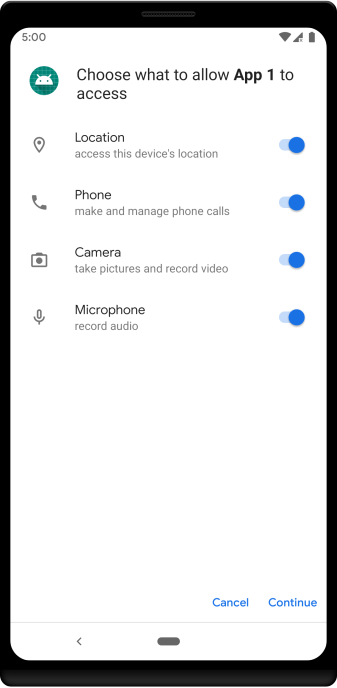
\includegraphics[width=.25\textwidth]{figure/chapter1/android3}\label{ch1:fig2:android3}}
\caption{The three Android permission models: install-time permission (all permissions are requested at install time); runtime-permission (permission can be delayed at the runtime); and the latest permission model (permissions can be requested at both the install time and runtime permission)}
\end{figure}

Although the newer permission models have allowed the applications to support knowledge to users for making security decisions, such changes do not guarantee that developers \emph{will} provide such knowledge. Indeed, we can always find news articles or forum posts complaining that Android permission purposes are confusing. As a result, we propose to study two problems: first, have Android apps provided sufficient knowledge supports for users' security decision making; second, if not enough knowledge are provided, how can we assist developers to improve the decision support. 

\textbf{Assisting Data Analytics for Business Decision Making}. A general strategy to support users' decision making, especially business decisions, is to support data analytics, including database queries. For example, the user may want to make a decision according to last years' sales record. On desktop/laptops, the decision making usually involves querying of a database. However, novel data analytics may not be familiar with SQL grammar. As a result, it would be convenient to support a natural language interface to assist the decision making. Figure~\ref{ch1:fig5:powerbi1} shows an example of such a natural language interface. When the user input the natural language question ``what is the breed of the dog named betty'', the system translates it into an SQL statement: \texttt{SELECT breed FROM dogs WHERE name = betty}, and displays the execution result. 

\begin{figure}[h]
\centering
\subfloat[][Conversational data analytics tool in Power BI (desktop)]{\includegraphics[width=.5\textwidth]{figure/chapter1/powerbi1_crop}\label{ch1:fig5:powerbi1}} \hskip 40pt
\subfloat[][Power BI iOS]{\includegraphics[width=.25\textwidth]{figure/chapter1/powerbi2}\label{ch1:fig5:powerbi2}} 
\caption{Microsoft Power BI interface (left) and the corresponding mobile application (right)}
\end{figure}

Mobile business intelligence is a new area (less than 10 years). However, surveys show that in 2017, 28\% percent of BI users stated that mobile BI was already in use in their company, with 23\% planned to be in use in the next 12 months and 22\% planned in the long term~\cite{mobilebi}. As of 2019, many mobile BI tools are in use. For example, Microsoft Power BI introduced the iOS application in 2015. Similar as the desktop version, the mobile applicaion also support the natural language interface feature (Figure~\ref{ch1:fig5:powerbi2}). 

To assist mobile users with business decision making, it thus is an important task to support natural language interface, i.e., translating the users' natural language question into SQL statement. Due to the aforementioned difficulty in mobile user interaction (i.e., small screen, difficulty researching information), it may be particularly difficult to write a correct SQL statement, therefore the support of natural language interface is particularly helpful. 

In these BI platforms, the NL2SQL must adapt to new database schemas provided by the user. As a result, the predictor must be able to generalize to new domains which has not been seen in the training data. The problem of cross-domain NL2SQL with complex query structure is still an active research area that has not been well solved. The problem of State-of-the-art approaches can achieve an accuracy of 65.5\%. As a result, we study the problem of translating natural language to SQL for cross-domain complex queries. 

\section{Organization of This Thesis}

The rest of this thesis is organized as follows. 

$\bullet$ \textbf{Chapter~\ref{ch2:shopping}: Assisting Shopping Decision Making with Numerical Faceted Search}. We study the problem of optimizing numerical facets to support users' shopping decision making on mobile devices. With a 2-month user query and click log on \url{www.walmart.com}, we develop a machine learning algorithm that suggests numerical ranges given a query. First, we propose an evaluation metric that evaluates the performance of a numerical range suggestion algorithm (Section~\ref{ch2:metric}). Based on the proposed metric, we propose three optimization algorithms by optimizing the metric directly (Section~\ref{ch2:dp}) and its upper bound (Section~\ref{ch2:percentage}). 

$\bullet$ \textbf{Chapter~\ref{ch3:runtime}: Empirical Study on Knowledge Support for Security Decision Making}. Before studying assisting users' mobile security decision making, we need to first empirically study whether existing applications have already provided sufficient explanations to support such decision making. Using sentence classification techniques, we creates a new dataset containing the explanation sentences by mobile applications. We propose five research questions to evaluate the sufficiency of explanations. Statistical significance tests show that generally, the decision support has not been sufficient compared with the suggestions by Android developers documentation. 

$\bullet$ \textbf{Chapter~\ref{ch4:clap}: Recommending Explanation to Assist Security Decision Making}. By identifying the deficiency in decision support, we propose to assist application developers to improve their existing explanations. By leveraging a large dataset containing the meta data of 1.45 million Playstore applications, we collect a large scale text corpus. By leveraging information retrieval techniques and unsupervised truth finding, our recommender system can suggest highly relevant sentences to the true purpose of the application. Qualitative evaluation shows the suggested sentences show three characteristics of interpretability. 

$\bullet$ \textbf{Chapter~\ref{ch5:nl2sql}: Assisting Business Decision Making with Natural Language to SQL Interface}. We study the problem of how to help mobile BI by supporting the natural language interface (NLI, or NL2SQL). We leverage a large complex cross-domain dataset named Spider to more closely simulate the scenario of mobile BI. By leveraging database values, we successfully matched database values that has been mentioned in the natural language question. We inject the matched database values to the existing state-of-the-art model on Spider, and observe 2.7\% improvement in the exact matching accuracy of output SQL statement. We further conduct an empirical study~\ref{ch5:sec:study} to explore potential ways for further improvement. 


\input{tex/2-shopping/2-shopping}

%!TEX root =../../thesis-ex.tex

\chapter{Empirical Study on Knowledge Support for Security Decision Making}
\label{ch3:runtime}

% Life's more fun when you live in the moment :) Happy Snapping!
%\vspace{-0.15in}
\section{Runtime Permission Rationale: Introduction}
\label{sec:intro}

%Android permission system controls user's private information (e.g., location) by engaging users to make security decisions. A successful permission system not only needs to sufficiently protect privacy, but should also support effective decision making by sufficiently educating users about why permissions are requested. 

Mobile security and privacy are two challenging tasks~\cite{journals/tocs/EnckGHTCCJMS14,conf/ccs/FeltCHSW11,conf/soups/FeltHEHCW12,conf/chi/AlmuhimediSSAAG15,conf/huc/LinSALHZ12,conf/soups/LinLSH14,yang2015appcontext}.
Recently user privacy issues gather tremendous attention after the Facebook-Cambridge Analytica data scandal~\cite{facebookleak}. 
Android's current solution for protecting the users' private data resources mainly relies on its sandbox mechanism and the permission system. 
Android permissions control the users' private data resources, e.g., locations and contact lists. 
The permission system regulates an Android app to request permissions, and the app users must grant these permissions before the app can get access to the users' sensitive data. 

In earlier versions of Android, permissions are requested at the installation time.
However, studies~\cite{conf/soups/FeltHEHCW12,conf/huc/LinSALHZ12} show that the install-time requests cannot effectively warn the users about potential security risks. 
The users are often not aware of the fact that permissions are requested, and the users also have poor understandings on the meanings and purposes of using the permissions~\cite{conf/soups/FeltHEHCW12,conf/fc/KelleyCCJSW12}. 
It is a critical task to educate the users by explaining permission purposes so that the users can better understand the purposes~\cite{conf/huc/LinSALHZ12,conf/uss/PanditaXYEX13,clap}.

% latex triming figures: \includegraphics[trim={5cm 0 0 0},clip]{example-image-a}
\begin{figure}[t]
	\vspace{-0.1in}
	\centering
	\subfloat[][Default permission-requesting message for the permission group \correcttexttt{STORAGE} in Android.]{\includegraphics[width=.45\linewidth]{figure/chapter2/intro-fig2.png}\label{fig:warning}}\hfill
	\subfloat[][A runtime-permission-group rationale provided by the app for the permission group \correcttexttt{LOCATION}.]{\includegraphics[width=.45\linewidth]{figure/chapter2/intro-fig1.jpg}\label{fig:rationale}}
	\caption{\label{fig:intro}}
	\vspace{-4ex}
\end{figure}

Since Android 6.0 (Marshmallow), the permission system has been replaced by a new system that requests permission groups~\cite{permgroup} at runtime. An example of runtime-permission-group requests is in Figure~\ref{fig:warning}, where Android shows the default permission-requesting message for the permission group \correcttexttt{STORAGE}\footnote{The permission-requesting message is the message displayed in the permission-requesting dialog (Figure~\ref{fig:warning}). For each permission group, this message is fixed across different apps. For example, the permission-requesting message for \correcttexttt{STORAGE} is \emph{Allow \textbf{appname} to access photos, media and files on your device?}}.
The runtime model has three advantages over the old model. 
(1) It gives the users more warnings than the install-time model. 
(2) It allows the users to control an app's privileges at the permission-group level. 
(3) It gives apps the opportunity to embed their permission-group requests in contexts, so that the requests are self-explanatory. 
For example, in Figure~\ref{fig:warning}, a request for accessing the user's gallery is prompted when she is about to send a Tweet. 

With the runtime-permission system, each Android app can leverage a dialog to provide a customized message for explaining its unique purpose of using the permission group.
In Figure~\ref{fig:rationale}, we show an example of such messages from the \emph{Facebook} app for explaining the purpose of requesting the user's location: ``\emph{Facebook uses this to make some features work...}''. 
Such customized messages are called \emph{runtime-permission-group rationales}. 
Runtime-permission-group rationales are often displayed before or after the permission-requesting messages, or upon the starting of the app. For the rest of this paper, for simplicity, whenever the context refers to a runtime-permission-group rationale or a runtime-permission-group request, we use the term \emph{rationale}, \emph{runtime rationale}, and \emph{permission-group rationale} in short for \emph{runtime-permission-group rationale}; we use the term \emph{permission request(-ing message)} in short for \emph{runtime-permission-group request(-ing message)}.

There are three main reasons why runtime rationales are useful in the new permission system. 
(1) \emph{Challenge in Explaining Background Purposes}. 
Although the runtime system allows permission-group requests to be self-explanatory in contexts, there exist cases where the permission groups are used in the background (e.g., read phone number, SMS)~\cite{Micinski2017UserIA}. 
As a result, there does not exist a user-aware context for asking such permission groups.
(2) \emph{Challenge in Explaining non-Straightforward Purposes}. 
When the purpose of requesting a permission group is not straightforward, such as when the permission group is not for achieving a  primary functionality, the context itself may not be clear enough to explain the purpose. 
For example, when the user is about to send a Tweet (Figure~\ref{fig:warning}), she may not notice that the location permission group is requested. 
(3) \emph{Effectiveness of Natural Language Explanations}. 
Prior work~\cite{conf/huc/LinSALHZ12} shows that the users find the usage of a permission better meets their expectation when the purpose of using such permission is explained with a natural language sentence. Furthermore, user studies~\cite{conf/chi/TanNTNTEW14} on Apple's iOS runtime-permission system also demonstrate that displaying runtime rationales can effectively increase the users' approval rates. 

The effectiveness of explaining permission purposes relies on the contents of the explanation sentences~\cite{conf/huc/LinSALHZ12}. 
Because the rationale sentences are created by apps, the quality of such rationales depends on how individual apps (developers) make decisions for providing rationales. 
Three essential decisions are  (1) which permission group(s) the app should explain the purposes for; (2) for each permission group, what words should be used for explaining the permission group's purpose; (3) how specific the explanation should be.

In this paper, we seek to answer the following questions: (1) what are the common decisions made by apps? (2) how are such decisions aligned with the goal of improving the users' understanding of permission-group purposes? 
To understand the general patterns of apps' permission-explaining behaviors, we conduct the first large-scale empirical study on runtime rationales. 
We collect an Android 6.0+ dataset consisting of 83,244 apps. 
From these apps, we obtain 115,558 rationale sentences. 
Our study focuses on the following five research questions.

{\bf RQ1: Overall Explanation Frequency}. We investigate the overall frequency for apps to explain permission-group purposes with rationales. The result can help us understand whether the developers generally acknowledge the usefulness of runtime rationales, and whether the users are generally warned for the usages of different permission groups. 

{\bf RQ2: Explanation Frequency for non-Straightforward vs. Straightforward Purposes}. Prior work~\cite{conf/codaspy/JingAZH14,conf/huc/LinSALHZ12} finds that the users have different expectations for different permission purposes. The Android official documentation~\cite{shouldshow} suggests that apps provide rationales when the permission group's purposes are not straightforward. Therefore, we investigate whether apps more frequently explain non-straightforward purposes than straightforward ones. The result can help us understand the helpfulness of rationales with the users' understandings of permission-group purposes. 

{\bf RQ3: Incorrect Rationales}. We study the population of rationales where the stated purpose is different from the true purpose, i.e., the rationales are incorrect. 
Such study is related to user expectation, because incorrect rationales may confuse the users and mislead them into making wrong security decisions. 

{\bf RQ4: Rationale Specificity}. How exactly do apps explain purposes of requesting permission groups? How much information do rationales carry? 
Do rationales provide more information than the permission-requesting message? 
Do apps provide more specific rationales for non-straightforward purposes than for straightforward purposes? 

{\bf RQ5: Rationales vs. App Descriptions}. Are apps that provide rationales more likely to explain the same permission group's purpose in the app description than apps that do not provide rationales? 
Are the behaviors of explaining a permission group's purposes consistent in the app description and in rationales? Do more apps explain their permission-group purposes in the app description than in rationales?

% In summary, we study the following five research questions:

% \textbf{RQ1}. How often do apps provide permission rationales?

% \textbf{RQ2}. Do apps provide more rationales for non-straightforward purposes or for straightforward ones?

% \textbf{RQ3}. Do there exist a significant number of incorrect rationales?

% \textbf{RQ4}. Do rationales tend to provide more specific information than the system-provided permission-requesting message?

% \textbf{RQ5}. How does explaining permissions in the rationales relate to explaining the same permissions in the app descriptions?


The rest of this paper is organized as follows. Section~\ref{sec:relwork} introduces background and related work, Section~\ref{sec:data} describes the data collection process. Sections~\ref{sec:rq1}-~\ref{sec:rq5} answer RQ1-RQ5. Sections~\ref{sec:threats}-~\ref{sec:conclusion} discuss threats to validity, implications, and conclusion of our study. 

%!TEX root =../main.tex

% Life's more fun when you live in the moment :) Happy Snapping!
\section{Background and Related Work}
\label{sec:relwork}

\textbf{Android Permissions and the Least-Privilege Principle}. A previous study~\cite{conf/ccs/FeltCHSW11} shows that compared with attack-performing malware, a more prevalent problem in the Android platform is the \emph{over-privilege} issue of Android permissions: apps often request more permissions than necessary. 
Felt \emph{et al.}~\cite{conf/soups/FeltHEHCW12} evaluate 940 apps and find that one-third of them are over-privileged. 
Existing work leverages  static-analysis techniques~\cite{conf/ccs/FeltCHSW11,conf/ccs/AuZHL12} and dynamic-analysis techniques~\cite{journals/tocs/EnckGHTCCJMS14} to build tools for analyzing whether an app follows the \emph{least-privilege principle}. 
The runtime-permission-group rationales we study are for helping the users make decisions on whether a permission-group request is over-privileged. 

\textbf{User Expectation}. Over time, the research literature on Android privacy has focused on studying whether and how an app's permission usage meets the users' expectation~\cite{conf/huc/LinSALHZ12,conf/icse/HuangZTWL14,conf/uss/PanditaXYEX13,conf/icse/GorlaTGZ14,conf/chi/AlmuhimediSSAAG15,Nissenbaum:2004,conf/uss/WijesekeraBHEWB15,conf/sp/RoesnerKMPWC12,conf/chi/KelleyCS13}. 
In particular, Lin \emph{et al.}~\cite{conf/huc/LinSALHZ12} find that the users' security concern for a permission depends on whether they can expect the permission usage. Jing \emph{et al.}~\cite{conf/codaspy/JingAZH14} further find that even in the same app, the users have different expectations for different permissions. For example, in the \emph{Skype} app, the users find the microphone permission more straightforward than the location permission. The Android official documentation~\cite{shouldshow} also points out this difference and suggests that app developers provide more runtime-permission-group rationales for purposes that are not straightforward to expect. 

The research literature on user expectation can be categorized into three lines of work. The first line of work is on detecting contradictions between the code behavior and the user interface~\cite{conf/icse/HuangZTWL14,conf/wisec/AndowALESX17}. The second line of work is on improving existing interfaces to enhance the users' awareness of permission usages~\cite{conf/chi/AlmuhimediSSAAG15,conf/sp/RoesnerKMPWC12,conf/huc/LiGC16,Nissenbaum:2004,Micinski2017UserIA,conf/uss/WijesekeraBHEWB15}. 
This line of work includes privacy nudging~\cite{conf/chi/AlmuhimediSSAAG15}, access control gadget~\cite{conf/sp/RoesnerKMPWC12}, and mapping between permissions and UI components~\cite{conf/huc/LiGC16}. 
In particular, Nissenbaum \emph{et al.}~\cite{Nissenbaum:2004} first propose the concept of privacy as the \emph{contextual integrity}; 
i.e., the users' decision-making process for privacy relies on the contexts~\cite{Micinski2017UserIA,conf/uss/WijesekeraBHEWB15,chen2013contextual,background}. 
The runtime-permission system incorporates the contextual integrity by allowing apps to ask for permission groups within the context. 
The third line of work is on using natural language sentences to represent or enhance the users' expectation regarding the permission usages~\cite{conf/huc/LinSALHZ12,conf/uss/PanditaXYEX13,conf/icse/GorlaTGZ14,conf/ccs/QuRZCZC14}. 
For example, Lin \emph{et al.}~\cite{conf/huc/LinSALHZ12} find that the users of an app are more comfortable with using the app when the app provides clarifications for the permission purposes than they do not provide such clarifications. 
Pandita \emph{et al.}~\cite{conf/uss/PanditaXYEX13} further extract permission explaining sentences from app descriptions. 
Our study results presented in Section~\ref{sec:rq5} show that apps explain purposes of requesting permission groups more frequently in the rationales than in the description. 

\textbf{Runtime Permission Groups and Runtime Rationales}. Since the launch of the runtime-permission system, another line of work~\cite{conf/soups/BonnePBT17,conf/huc/LinSALHZ12,conf/chi/TanNTNTEW14} (including our work) focuses on the runtime-permission system and the users' decisions on such system. 
In particular, Bonne \emph{et al.}~\cite{conf/soups/BonnePBT17} conduct a study similar to the study by Lin \emph{et al.}~\cite{conf/huc/LinSALHZ12} under the runtime-permission system, showing the users' security decisions in the runtime system also rely on their expectations of the permission usages. 
The closest to our work is the study by Tan \emph{et al.}~\cite{conf/chi/TanNTNTEW14} on the effects of runtime rationales in the iOS system. 
Their user-study results show that rationales can improve the users' approval rates for permission requests and increase the comfortableness for the users to use the app. 
Although they have not observed a significant correlation between the rationale contents and the approval rates, such observations may be due to the fact that only one fake app is examined with limited user feedback. 
As a result, such unrelatedness cannot be trivially generalized to our case. Wijesekera et al.~\cite{conf/sp/WijesekeraBTREW17} redesigns the timing of runtime prompts to reduce the \emph{satisficing} and \emph{habituation} issues~\cite{conf/www/AkhaweAVS13,Wogalter2002ResearchbasedGF,harbach2013sorry,conf/soups/SchaubBDC15}. 
Both Wijesekera \emph{et al.}~\cite{conf/sp/WijesekeraBTREW17} and Olejnik \emph{et al.}~\cite{conf/sp/OlejnikDMHKH17} leverage machine learning techniques to reduce user efforts in making decisions for permission requests. 

%!TEX root =../main.tex

% Life's more fun when you live in the moment :) Happy Snapping!
\vspace{-0.1in}
\section{Data Collection}
\label{sec:data}

\vspace{-0.07in}
\subsection{Crawling Apps}

Since the launch of Android 6.0, many apps have migrated to support the newer versions of Android. 
To obtain as many Android 6.0+ apps as possible, we crawl apps from the following two sources: 
(1) we crawl the top-500 apps in each category from the Google Play store, obtaining 23,779 apps in total; 
(2) we crawl 482,591 apps from APKPure~\cite{apkpure}, which is another app store with copied apps (same ID, same category, same description, etc.) from the Google Play store\footnote{We are not able to collect all these apps from the Google Play store, due to its anti-theft protection that limits the downloading scale.}. 
From the two sources, we collect 494,758 apps. Among these apps, we find 83,244 apps that 
(1) contain version(s) under Android 6.0+; 
(2) request at least 1 out of the 9 dangerous permission groups (Table~\ref{tab:permission}). 
We use these 83,244 apps as the dataset in this paper\footnote{To the best of our knowledge, this dataset is the largest app collection on runtime rationales; 
it is orders of magnitude larger than other runtime-rationale collections in existing work~\cite{Micinski2017UserIA,conf/chi/TanNTNTEW14}.}. 

\subsection{Annotating Permission-group Rationales}

For each app found in the preceding step, we annotate and extract runtime rationales from the app. 
Same as other static user interface texts, runtime rationales are stored in an app's \correcttexttt{./res/values/strings.xml} file. 
Each line of this file contains a rationale's name and the content of the rationale. 

The size of our dataset dictates that it is intractable to manually annotate all the string variables. 
As a result, we leverage two automatic sentence-annotating techniques: 
(1) keyword matching; 
(2) CNN sentence classifier. 
The automatic annotation is a two-step process. 

\textbf{Annotating Rationales for All Permission Groups}. 
For the first step, we design a keyword matching technique to annotate whether a string variable contains mentions of a permission group. 
More specifically, we assign a binary label to each string variable by matching the variable's name or content against 18 keywords referring to permission groups, including ``\emph{permission}'', ``\emph{rationale}'', and ``\emph{toast}''\footnote{The complete list of the 18 keywords can be found on our project website~\cite{runtimeproj}.}. 
To estimate the recall of keyword matching, we randomly sample 10 apps and inspect their string resource files. 
The result of our inspection shows that such keyword matching found all the rationales in the 10 apps. 

\textbf{Annotating Rationales for the 8 Dangerous Permission Groups}\footnote{In this paper, we skip the \correcttexttt{BODY\_SENSORS} permission group because it contains too few rationales.}. 
For the second step, we use the CNN sentence classifier~\cite{cnn,kim2014convolutional} to annotate the outputs from the first step. The annotations indicate whether each rationale describes 1 of the 9 dangerous permission groups~\cite{permgroup}. 
The 9 permission groups contain 26 permissions. These permission groups' protection levels are dangerous and the purposes of requesting these permission groups are relatively straightforward for the users to understand. 
For each permission group, we train a different CNN sentence classifier. 
We manually annotate 200$\sim$700 rationales as the training examples for each classifier. 
After applying CNN, we estimate the classifier's false positive rate (FP) and false negative rate (FN) by inspecting 100 output examples in each permission group. The average FP (FN) over the 8 permission groups is 5.1\% (6.8\%) and the maximum FP (FN) is 13\% (16\%). In total, CNN annotates 115,558 rationales, which can be found on our project's website~\cite{runtimeproj}. 

\textbf{Discussion}. One caveat of our data collection process is that the rationales in string resource files are only \emph{candidates} for runtime prompts. 
That is, they may not be displayed to the users. 
The reason why we do not study only the actually-displayed rationales is that such study relies on dynamic-analysis techniques, which limit the scale of our study subjects.

\section{RQ1: Overall Explanation Frequency}
\label{sec:rq1}

In the first step of our study, we investigate the proportion of apps that provide permission-group rationales to answer RQ1: how often do apps provide permission-group rationales?  
For each of the 9 permission groups, we count how many apps in our dataset request the permission group; 
we denote this value as \textsf{\#used apps}. Among these apps, we further count how many of them explain the requested permission group's purposes with rationales; 
we denote this value as \textsf{\#explained apps}. Given the two values, we measure the \emph{explanation proportion} of a group of apps:

\begin{mydef}[Explanation proportion]
Given a group of apps, its explanation proportion of a permission group is the proportion of apps in that group to explain the purposes of requesting the permission group,  
i.e., \textsf{\#explained apps} / \textsf{\#used apps}. We denote the explanation proportion as \textsf{\%exp}. 
\end{mydef}

\begin{table}[t]
\centering
\caption{The number of the used apps (the \textsf{\#used apps} column), the explained apps (the \textsf{\#explained apps} column), and the proportion of explained app in the used apps (the \textsf{\%exp} column). We sort the permission groups by \textsf{\#used apps}. \label{tab:permission}}
\begin{tabular}{|l|r|r|r|r|r|r|r|}
\hline
\multirow{2}{*}{permgroup}  & \textsf{\#used} &  \textsf{\#explain}  & \multirow{2}{*}{\textsf{\%exp}} & \textsf{\%exp} \\
& \textsf{apps} & \textsf{-ed apps} & & (top) \\
\hline\hline
\correcttexttt{STORAGE} & 73,031 & 14,668 & 20.2\% & \textbf{28.3\%} \\ \hline
\correcttexttt{LOCATION} & 32,648 & 7,088 & \textbf{21.6\%} & \textbf{30.7\%} \\ \hline
\correcttexttt{PHONE} & 31,198& 2,070 &6.7\% & 11.0\% \\ \hline
\correcttexttt{CONTACTS} & 23,492& 2,607 & 11.1\% & 17.7\%\\ \hline
\correcttexttt{CAMERA} & 16,557& 4,235 &\textbf{25.6\%} & \textbf{37.7\%} \\ \hline
\correcttexttt{MICROPHONE} & 9,130& 2,152 & \textbf{23.5\%} & 28.0\%\\ \hline
\correcttexttt{SMS} & 4,589 & 589  & 12.8\% & 16.0\% \\ \hline
\correcttexttt{CALENDAR} & 2,492 & 357 & 14.2\% & 22.6\%\\ \hline
\correcttexttt{BODY\_SENSORS} & 122  & 16  & 13.1\% & 15.4\% \\ \hline
overall & 83,244 & 19,879 & 23.8\% & 33.9\% \\ \hline
\end{tabular}
\vspace{-0.15in}
\end{table}

In Table~\ref{tab:permission}, we show the values of \textsf{\#used apps}, \textsf{\#explained apps}, and \textsf{\%exp} for each permission group. 
In addition, we compute the \textsf{\%exp} value for only the categorical top-500 apps; we denote this value as \textsf{\%exp} (top). 

{\bf Result Analysis}. From Table~\ref{tab:permission} we can observe three findings.
(1) Overall, 23.8\% apps provide runtime rationale. 
(2) The top-500 apps more frequently explain the purposes of using permission groups than the overall apps do.  
(3) The purposes of the four permission groups \correcttexttt{STORAGE}, \correcttexttt{LOCATION}, \correcttexttt{CAMERA}, and \correcttexttt{MICROPHONE} are more frequently explained than the other five permission groups. 

{\bf Finding Summary for RQ1}. 23.8\% apps provide runtime rationales for their permission-group requests. 
Among all the permission groups, four groups' purposes are explained more often than the other permission groups. This result may imply that app developers are less familiar with the purposes of \correcttexttt{PHONE} and \correcttexttt{CONTACTS}. 

\section{RQ2: Explanation Frequency for Non-straightforward vs. Straightforward Purposes}
\label{sec:rq2}

In the second part of our study, we seek to \emph{quantitatively} answer RQ2: 
do apps provide more rationales for non-straightforward permission-group purposes than for straightforward permission-group purposes? 

It is challenging to \emph{precisely} measure the straightforwardness for understanding the purpose of requesting a permission group. 
The reason for such challenge is that such straightforwardness relies on each user's existing knowledge, which varies from user to user. Therefore, we propose to \emph{approximate} the straightforwardness by measuring the \emph{usage proportion} of a permission group in \emph{a set of apps}:

\begin{mydef}[Usage proportion]
Given a set of apps, its usage proportion (denoted as  \textsf{\%use}) of a permission group  is the proportion of the apps (in this set) that request the permission group. 
\label{def:usagefreq}
\end{mydef}

Our approximation is based on the observation that if a permission group is frequently used by a set of apps, the permission-group purpose in that app set is often also straightforward to understand. 
For example, in a camera app, the users are more likely to understand the purpose of the camera permission group than the location permission group~\cite{shouldshow}; 
meanwhile, our statistics show that camera apps also more frequently request the camera permission group (71.4\%) than the location permission group (27.0\%). 

\begin{table}[t]
\centering
\caption{The app sets for measuring the correlation between the usage proportion and the explanation proportion. The apps in each set share the same purpose (the purpose column) to use the primary permission group (the permgroup column) with the usage proportion (the \textsf{\%use} column).\label{tab:appgroup}}
\begin{tabular}{|c|c|c|c|r|}
\hline
% 985*323  &  176*248  &  393*223  &  189*67  &  173*138  &  105*313  &  24*216  &  12*136  &
% 771*252  &  906*318  &  226*250  &  366*94  &  308*124  &  67*199  &  70*117  &  41*144  & 
% 749*309  &  234*380  &  798*276  &  235*57  &  185*95  &  215*331  &  49*0  &  9*91  &  
% 759*180  &  286*244  &  274*149  &  841*238  &  552*198  &  302*184  &  347*77  &  21*74  & 
% 772*258  &  349*205  &  187*233  &  668*185  &  833*260  &  156*194  &  386*84  &  61*286  &  
% 882*318  &  293*291  &  255*249  &  527*186  &  418*186  &  758*179  &  147*147  &  26*167  &
% 706*164  &  326*83  &  205*92  &  628*167  &  625*211  &  105*154  &  604*170  &  27*0  & 
% 783*179  &  340*186  &  143*186  &  277*133  &  353*142  &  37*182  &  43*77  &  360*222  &
appset & permgroup & purpose & \textsf{\%use} & \textsf{\#apps}\\ \hline\hline
 file mgr& \correcttexttt{STORAGE} & file managing & 95.4\%& 499\\\hline
 video players & \correcttexttt{STORAGE}& store video  & 96.6\% & 1,306\\ \hline
 photography & \correcttexttt{STORAGE}& store photos  & 99.7\% & 3,534\\ \hline\hline
%1: 954*349  &  220*255  &  154*299  &  305*145  &  381*289  &  0*0  &  126*286  &  62*226  & 
%2: 962*338  &  211*207  &  240*361  &  268*89  &  241*86  &  218*291  &  31*200  &  11*67  &
%3: 997*314  &  156*268  &  484*193  &  143*28  &  118*108  &  71*327  &  6*45  &  6*50  &
%all: 985*323  &  176*248  &  393*223  &  189*67  &  173*138  &  105*313  &  24*216  &  12*136  &
% 5319
 maps\&navi & \correcttexttt{LOCATION}& GPS navigation  & 92.6\% & 1,541\\ \hline
 weather & \correcttexttt{LOCATION}& local weather  & 95.4\% & 908\\ \hline
travel\&local  & \correcttexttt{LOCATION}& \makecell{local search} & 87.8\% & 2,647\\ \hline\hline
% 1: 816*244  &  878*316  &  299*255  &  400*88  &  376*115  &  90*218  &  71*134  &  63*138  &  
% 2: 742*378  &  954*367  &  52*298  &  313*99  &  134*41  &  12*182  &  8*0  &  10*222  & 
% 3: 816*244  &  878*316  &  299*255  &  400*88  &  376*115  &  90*218  &  71*134  &  63*138  & 
% all: 771*252  &  906*318  &  226*250  &  366*94  &  308*124  &  67*199  &  70*117  &  41*144  &  
% 5096
lockscreen & \correcttexttt{PHONE} & \makecell{answer call wh\\-en screen locked} & 82.6\% & 425\\ \hline
voip call & \correcttexttt{PHONE} & \makecell{make calls} & 84.9\% & 847\\ \hline
caller id & \correcttexttt{PHONE} & \makecell{caller id} & 92.0\% & 175 \\ \hline\hline
% 1: 774*149  &  205*391  &  256*46  &  826*197  &  155*30  &  24*0  &  144*16  &  19*0  &  
% 2: 751*197  &  327*199  &  282*197  &  849*260  &  750*214  &  442*190  &  451*86  &  22*105  &  
% 3: 686*117  &  474*96  &  211*54  &  920*130  &  886*161  &  251*136  &  663*52  &  34*167  &
% all: 759*180  &  286*244  &  274*149  &  841*238  &  552*198  &  302*184  &  347*77  &  21*74  &  
% 1274
caller id & \correcttexttt{CONTACTS} & \makecell{caller id} & 86.7\% & 196 \\ \hline
mail & \correcttexttt{CONTACTS} & auto complete & 77.1\% & 140 \\ \hline
contacts & \correcttexttt{CONTACTS} & contacts backup & 85.8\% & 259 \\ \hline\hline
% 1: 704*123  &  485*137  &  214*71  &  908*129  &  867*165  &  235*130  &  633*56  &  36*143  &  
% 2: 879*431  &  264*324  &  179*520  &  386*296  &  771*361  &  143*350  &  164*87  &  121*353  &
% 3: 722*176  &  340*216  &  220*140  &  757*168  &  857*216  &  131*147  &  440*114  &  35*222  & 
% all: 772*258  &  349*205  &  187*233  &  668*185  &  833*260  &  156*194  &  386*84  &  61*286  & 
% 461
flashlight & \correcttexttt{CAMERA} & flashlight & 96.6\% & 298 \\ \hline
qrscan & \correcttexttt{CAMERA} & qr scanner & 88.4\% & 155 \\ \hline
camera & \correcttexttt{CAMERA} & selfie\&camera & 71.4\% & 749 \\ \hline\hline
% 1: 282*60  &  134*125  &  966*174  &  272*74  &  111*0  &  77*174  &  131*0  &  7*0  & 
% 2: 755*393  &  245*263  &  884*445  &  239*135  &  342*170  &  58*556  &  19*0  &  39*167  &
% 3: 933*325  &  270*450  &  714*286  &  219*30  &  183*88  &  303*339  &  23*0  &  4*0  &  
% all: 749*309  &  234*380  &  798*276  &  235*57  &  185*95  &  215*331  &  49*0  &  9*91  & 
% 1193
recorder & \correcttexttt{MIC} & voice recorder & 75.7\% & 559 \\ \hline
video chat & \correcttexttt{MIC} & video chat & 77.0\% & 139 \\ \hline\hline
% 1: 880*317  &  240*284  &  123*174  &  492*193  &  386*153  &  757*168  &  111*161  &  27*133  &
% 2: 892*331  &  525*315  &  813*310  &  676*191  &  554*286  &  770*243  &  317*136  &  22*333  &  
% all: 882*318  &  293*291  &  255*249  &  527*186  &  418*186  &  758*179  &  147*147  &  26*167  &
% 693 
sms & \correcttexttt{SMS} & sms & 60.4\% & 379\\ \hline
% all: 706*164  &  326*83  &  205*92  &  628*167  &  625*211  &  105*154  &  604*170  &  27*0  & 
calendar & \correcttexttt{CALEND} & calendar & 36.0\% & 300 \\ \hline
% all: 783*179  &  340*186  &  143*186  &  277*133  &  353*142  &  37*182  &  43*77  &  360*222  &
\end{tabular}
\vspace{-0.15in}
\end{table}

\begin{figure} 
\vspace{-0.15in}
    \centering
  \subfloat{%
   \vspace{-0.2in}
       \includegraphics[width=0.85\linewidth]{figure/chapter2/use_mat.pdf}}\\
    \vspace{-0.15in}
     \subfloat{%
       \includegraphics[width=0.85\linewidth]{figure/chapter2/exp_mat.pdf}}
\caption{The usage proportion (top) and the explanation proportion (bottom) of the app sets in Table~\ref{tab:appgroup}. Each element at ($Q$, $P$) shows the proportion of apps in set $Q$ to use/explain the purpose of permission group $P$.\label{fig:mat}}
\vspace{-0.2in}
\end{figure}

To answer RQ2, we first introduce the definitions of the primary permission group. 

\begin{mydef}[Primary Permission Group]
Given a set of apps that share the same primary functionality, if any app relies on (does not rely on) requesting a permission group to achieve that primary functionality, we say that this permission group is a primary (non-primary) permission group to this app set, and this app set is a primary (non-primary) app set to this permission group. An example of such primary (non-primary) pairs is GPS navigation apps and \correcttexttt{LOCATION} (\correcttexttt{CAMERA}) permission group. 
\end{mydef}

To study the relation between the straightforwardness of permission-group purposes and explanation proportions, we leverage the following three-step process. (1) For each permission group $P$, we use keyword matching to identify 1$\sim$3 app sets such that $P$ is a primary permission group to these app sets. (2) For each permission group $Q$, we merge its primary app sets to obtain a larger primary app set for $Q$. (3) For each permission group $P$ and the merged app sets for each permission group $Q$, we compute the proportion for app set $Q$ to use/explain $P$, obtaining two 8 $\times$ 8 matrices. We show all the app sets in Table~\ref{tab:appgroup}, and the two matrices in Figure~\ref{fig:mat}. In each matrix in Figure~\ref{fig:mat}, each row corresponds to a merged app set $Q$ and each column corresponds to a permission group $P$. For each row/column, we also compute the average over its off-diagonal elements and show these values in an additional column/row named \textsf{off-Diag}. That is, elements in \textsf{off-Diag} show the average over non-primary permission groups/app sets.

{\bf Why Using Primary Permission Groups?} By introducing primary permission groups, we are able to identify permission-group purposes that are clearly straightforward (Table~\ref{tab:appgroup}), so that the boundaries between straightforward purposes and non-straightforward purposes are relatively well defined. We can observe such boundaries from the usage proportion matrix (Figure~\ref{fig:mat}, top).  
% storage: 0.4414246482539629, 0.008964284305333605
% camera: -0.48974301374955836, 0.028389953739503194
% location: 0.6145077501985943, 0.0013987271797970303
% phone: 0.5070562990412617, 0.06422788746797548
% contact: 0.7579019068029721, 0.0010614524201611319
% mic: 0.17164627894918055, 0.5407508597319843

\begin{table}[t]
\centering
\vspace{-0.05in}
\caption{The Pearson correlation tests of each permission group, between the usage proportion and the explanation proportion on the 35 Play-store app sets. \label{tab:cate}}
\begin{tabular}{|p{0.2cm}|p{0.5cm}|p{0.13cm}|p{0.5cm}|p{0.13cm}|p{0.5cm}|p{0.13cm}|p{0.5cm}|p{0.33cm}|p{0.5cm}|p{0.13cm}|p{0.13cm}|}
\hline
\multicolumn{2}{|c|}{\correcttexttt{STORAGE}}  & \multicolumn{2}{c|}{\correcttexttt{LOC}}  & \multicolumn{2}{c|}{\correcttexttt{PHONE}} & \multicolumn{2}{c|}{\correcttexttt{CONTACT}} & \multicolumn{2}{c|}{\correcttexttt{CAMERA}} & \multicolumn{2}{c|}{\correcttexttt{MIC}} \\ \hline\hline
r & p & r & p &r & p &r & p &r & p &r & p  \\ \hline
.4 & 8e-3 & .6 & 1e-3  & .5 & 6e-2 & .8 & 1e-3 & {-.5} & 2e-2 & .2 & .5\\ \hline
 \end{tabular}
 \vspace{-0.1in}
 \end{table}

{\bf Result Analysis}. We can observe the following findings from the explanation matrix in Figure~\ref{fig:mat} (bottom). 
(1) By comparing every diagonal element with its two \textsf{off-Diag} counterparts, we can observe that the diagonal elements are usually larger, indicating that straightforward permission-group purposes are explained more frequently than non-straightforward ones. 
On the other hand, there exist a few exceptional cases in \correcttexttt{LOCATION}, \correcttexttt{MICROPHONE}, \correcttexttt{SMS}, and \correcttexttt{CALENDAR} where at least one off-diagonal element is larger than the diagonal element, indicating that non-straightforward permission-group purposes are explained more frequently in these cases. 
(2) By comparing the elements in the \textsf{off-Diag} row, we find that the permission groups for which non-straightforward purposes are most explained are \correcttexttt{STORAGE}, \correcttexttt{LOCATION}, \correcttexttt{CAMERA}, and \correcttexttt{MICROPHONE}. 
Such result is consistent with the overall explanation proportions in Table~\ref{tab:permission}.

% to be added to the extended version:
\textbf{Measuring Correlation Over All Apps}. Because the app sets in Table~\ref{tab:appgroup} cover only a subset of apps, we further design the second measurement study to capture all apps in our dataset. 
The second study includes the following two-step process. 
(1) Based on the app categories in the Google Play store, we partition all apps into 35 sets. After the partition, the two permission groups \correcttexttt{SMS} and \correcttexttt{CALENDAR} contain too few rationales in each app set, and therefore we discard these two permission groups. 
(2) For each permission group, we compute all its usage proportions and explanation proportions in the 35 app sets, and test the Pearson correlation coefficient~\cite{pearson} between the usage proportions and explanation proportions. 
In Table~\ref{tab:cate}, we show the results of the Pearson tests. We can observe that 4 out of the 6 tests show significantly positive correlation, i.e., straightforward purposes are usually more frequently explained. 
Such results are generally consistent with the results in Figure~\ref{fig:mat}. 

\textbf{Finding Summary for RQ2}. Overall, apps \emph{have not} provided more runtime rationales for non-straightforward permission-group purposes than for straightforward ones except for a few cases. This result implies that the majority of apps \emph{have not} followed the suggestion from the Android official documentation~\cite{shouldshow} to provide rationales for non-straightforward permission-group purposes.

\section{RQ3: Incorrect Rationales}
\label{sec:rq3}

In the third part of our study, we investigate the correctness of permission-group rationales. 
We seek to answer RQ3: does there exist a significant proportion of runtime rationales where the stated purposes do not match the true purposes?
%what is the extent of incorrect rationales?
%are there rationales that state one purpose but use the permission group for a different purpose?

It is challenging to derive an app's true purpose for requesting a permission group. However, we can coarsely differentiate between purposes by checking the permissions under a permission group. 
Among the 9 permission groups in Android 6.0 and higher versions, 6 permission groups each contain more than one permission~\cite{permgroup}. For example, the \correcttexttt{PHONE} permission group controls the access to phone-call-related sensitive resources, and this permission group contains 9 phone-call-related permissions: \correcttexttt{CALL\_PHONE}, \correcttexttt{READ\_CALL\_LOG}, \correcttexttt{READ\_PHONE\_STATE}, etc. By examining whether the app requests \correcttexttt{READ\_CALL\_LOG} or \correcttexttt{READ\_PHONE\_STATE}, we can differentiate between the purposes of reading the user's call logs and accessing the user's phone number. 

In order to easily identify the mismatches between the stated purpose and the true purpose, we study 3 permission groups consisting of relatively diverse permissions: \correcttexttt{PHONE}, \correcttexttt{CONTACTS}, and \correcttexttt{LOCATION}. 
In particular, each of the 3 groups contains 1 permission such that 90\% apps requesting the group have requested that permission (whereas other permissions in the same group are requested less frequently);  therefore, we name such permission a \emph{basic permission}. 
The basic permissions of \correcttexttt{PHONE}, \correcttexttt{CONTACTS}, and \correcttexttt{LOCATION} are \correcttexttt{READ\_PHONE\_STATE}, \correcttexttt{GET\_ACCOUNTS}, and \correcttexttt{ACCESS\_COARSE\_LOCATION}, respectively. 

\begin{mydef}[Apps with Incorrect Rationales]
We identify two cases for an app to contain incorrect rationale(s): 
(1) all the rationales state that the app requests only the basic permission, but in fact, the app has requested other permissions (in the same permission group); 
(2) the app requests only the basic permission, but it contains some rationales stating that it has requested other permissions (in the same permission group). 
\end{mydef}

How many apps does each of the two incorrect cases contains? Both cases can mislead the user to make wrong decisions. 
For case (1), the user may grant the permission-group request with the belief that she has granted only the basic permission, but in fact she has granted other permissions. 
For case (2), the user may deny the permission-group request, because the stated purpose of such permission group seems to be unrelated to the app's functionality, 
e.g., when a music player app requests the \correcttexttt{READ\_PHONE\_STATE} permission only to pause the music when receiving phone calls, 
the rationale can raise the user's security concern by stating that the music app needs to make a phone call. 
After the user denies the phone permission group, the app also loses the access to pausing the music. 

\begin{table}[t]
\centering
\caption{The upper table shows the criteria for annotating the basic permission and other permissions in the same permission group. The lower table shows the estimated lower bounds on the numbers of apps containing incorrectly stated rationales. \label{tab:lower}}
\begin{tabular}{|c|c|c|c|c|c|c|c|}
\hline
\multicolumn{2}{|c|}{} & \multicolumn{2}{c|}{\correcttexttt{CONTACTS}} & \multicolumn{2}{c|}{\correcttexttt{PHONE}} & \multicolumn{2}{c|}{\correcttexttt{LOCATION}} \\ \hline\hline
 \multirow{3}{*}{\makecell{annotate\\criterion}} & \makecell{basic per\\-mission\\class (a)} & \multicolumn{2}{c|}{\makecell{google \\account/\\sign in/\\email add\\ dress}} & \multicolumn{2}{c|}{\makecell{pause inc\\ oming call/\\imei/ ident\\ity/ number/\\cellular}} & \multicolumn{2}{c|}{\makecell{coarse loc\\/area/region\\/approximate\\/beacon\\ /country}}\\ \cline{2-8}
 & \makecell{other per-\\missions\\class (b)} & \multicolumn{2}{c|}{\makecell{contacts/\\friends/\\phonebook}}& \multicolumn{2}{c|}{\makecell{make call/\\call phone/\\call logs}}& \multicolumn{2}{c|}{\makecell{driving/\\fine loc/\\coordinate}}\\ \hline\hline
 \multirow{4}{*}{\makecell{incorrect\\apps}} & \multirow{2}{*}{\makecell{case (1)}} & \textsf{\#err} & \textsf{\%err} & \textsf{\#err}& \textsf{\%err} & \textsf{\#err} & \textsf{\%err} \\ \cline{3-8}
 & & 93& 4.6& 139& 11.3& 9& 0.1\\ \cline{2-8}
 & \multirow{2}{*}{\makecell{case (2)}} & \textsf{\#err} & \textsf{\%err} & \textsf{\#err} & \textsf{\%err} & \textsf{\#err} & \textsf{\%err} \\ \cline{3-8}
 & & 76 & 13.2 & 37& 4.2 & 3& 0.6\\ \hline
 \end{tabular}
 \vspace{-0.15in}
 \end{table}

To study the populations of the two preceding incorrect cases, we again leverage the aforementioned CNN sentence classifier~\cite{cnn}. 
We classify each runtime rationale into one of the following three classes: 
(a) the rationale states the purpose of requesting a basic permission; 
(b) the rationale states the purpose of requesting a permission other than the basic permission; (c) neither (a) nor (b). 
For each of the three permission groups, we manually annotate 600$\sim$900 rationales as the training data. 
After we obtain the predicted labels, we manually judge the resulting rationales that are predicted as (a) or (b) to make sure that there do not exist false positive annotations for incorrect case (1) or (2). 
In Table~\ref{tab:lower}, we show the lower-bound estimations (\textsf{\#err} and \textsf{\%err}) of the two incorrect cases' populations. 
We also show the detailed criteria of our annotations for (a) and (b). 
The list of incorrect rationales and their apps can be found on our project website~\cite{runtimeproj}.

{\bf Result Analysis}. From Table~\ref{tab:lower} we can observe that there exist a significant proportion of incorrectly stated runtime rationales, especially in the incorrect case (1) of the phone permission group and the incorrect case (2) of the contacts permission group. 
In contrast, there exist fewer incorrect cases in the location permission group.
The reason for the location permission group to contain fewer incorrect cases may be that the majority of apps claim only the usage of location, without specifying whether the requested location is fine or coarse. 
The contacts and phone permission groups contain more diverse purposes than the location group does, and our study results show that a significant proportion of apps requesting the two groups state the wrong purposes. 
For example, a significant number of FM radio apps state in the rationales that these apps \emph{only} need to use the phone state to pause the radio when receiving incoming calls;  
however, these apps have also requested the \correcttexttt{CALL\_PHONE} permission, indicating that if the user grants the permission group, these apps also gain the access to \emph{making phone calls} within the app. 

{\bf Finding Summary for RQ3}. There exist a significant proportion of incorrect runtime rationales for the \correcttexttt{CONTACTS} and the \correcttexttt{PHONE} permission groups. This result implies that apps may have confused the users by stating the incorrect permission-group purposes for \correcttexttt{PHONE} and \correcttexttt{CONTACTS}. 

\vspace{-0.05in}
\section{RQ4: Rationale Specificity}
\label{sec:rq4}

In the fourth part of our study, we look into the informativeness of runtime rationales. 
In particular, we seek to answer RQ4: do rationales (e.g., the rationale in Figure~\ref{fig:rationale}) provide more specific information than the system-provided permission-requesting messages (e.g., the message in Figure~\ref{fig:warning})?

% Whenever an app requests 1 of the 9 permission groups for the first time, Android displays a fixed system message for each permission group. 
% For example, the permission-requesting message for the \correcttexttt{STORAGE} permission group is always ``\emph{Allow appname to access photos, media, and files on your device?}''. 
% This message states only the fact that the app is requesting the storage permission group, without providing further information on the specific functionality that causes the app to request the permission group. 

\begin{mydef}[Redundant Rationales]
If a runtime rationale states only the fact that the app is requesting the permission group, i.e., it does not provide more information than the permission-requesting message, we say that the rationale is redundant, and otherwise non-redundant. 
\end{mydef}

Among all the runtime rationales, how many are non-redundant ones? How much do the proportions of non-redundant rationales in each permission group vary across  permission groups?

\begin{figure}[t]
\vspace{-0.13in}
\centering
\begin{tikzpicture} [scale=.9]
\begin{groupplot}[group style={group size= 1 by 2},height=5cm,width=7cm]%[ybar stacked,xtick=\empty,]%ytick=\empty]
\nextgroupplot[ybar,symbolic x coords={3,13, 23, 33, 43, 53}, ybar=.05cm, legend style={at={(1.25, 0.9),font=\small},anchor=north, cells={align=left}}, enlarge x limits=0.1, ymin=0, ymax=1.0,ymajorgrids = true,bar width = 4.5,xtick=data,xticklabels={storage, locate, contact, phone, cam, mic}, xticklabel style={rotate=90}]%ytick=\empty]
\addplot[fill=white,draw=black] 
coordinates {(3, 0.5063)  (13, 0.4626) (23, 0.6301) (33, 0.8426) (43, 0.5456)  (53, 0.2000)};
\addplot[fill=blue,draw=blue] 
coordinates {(3, 0.5776) (13, 0.3666) (23, 0.7210) (33, 0.7242) (43, 0.5441)  (53, 0.2320)};
\addplot[fill=black,draw=black] 
coordinates {(3, 0.5389) (13, 0.4251) (23, 0.7020) (33, 0.7744)  (43, 0.5444)  (53, 0.2270)};
\addlegendentry{primary \\permission\\ group}
\addlegendentry{non-primary\\permission\\ group}
\addlegendentry{overall}
\end{groupplot}
\end{tikzpicture}
\vspace{-0.1in}
\caption{The proportions of non-redundant rationales.\label{fig:nonredunt}}
\vspace{-0.22in}
\end{figure}

To study the population of non-redundant rationales, we leverage the named entity tagging (NER) technique~\cite{conf/acl/FinkelGM05}. 
The reason for us to leverage the NER technique is our observation that non-redundant rationales usually use some words to state the more specific purposes than the fact of using the permission group. 
Moreover, these purpose-stating words usually appear in textual patterns. 
As a result, we can leverage such textual patterns to detect non-redundant rationales. 
For example, in the following rationale, the words tagged with ``\emph{S}'' explain the \emph{specific} purpose of using the permission group \correcttexttt{PHONE}, and the words tagged with \emph{\_O} are other words: ``\emph{this\_O radio\_O application\_O would\_O like\_O to\_O use\_O the\_O phone\_O permission\_O to\_S pause\_S the\_S radio\_S when\_S receiving\_S incoming\_S calls\_S}''. We train a different NER tagger for each of the top-6 permission groups in Table~\ref{tab:permission}\footnote{We skip \correcttexttt{SMS} and \correcttexttt{CALENDAR}, because they both contain too few rationales for estimating the proportions of non-redundant rationales.}. 
For each permission group, we manually annotate 200$\sim$1,000 training examples.
To evaluate the performance of our NER tagger, we randomly sample 100 rationales from NER's output for each permission group, and manually judge these sampled rationales. 
Our judgment results show that NER's prediction accuracy ranges from 85\% to 94\%. The lists of redundant and non-redundant rationales tagged by NER can be found on our project website~\cite{runtimeproj}. 
Next, we obtain the proportions of non-redundant rationales in each permission group. We plot these proportions in Figure~\ref{fig:nonredunt}.

{\bf Result Analysis}. We can observe three findings from Figure~\ref{fig:nonredunt} and additional experiments. 
(1) The proportions of redundant runtime rationales range from 23\% to 77\%. 
(2) While the two permission groups \correcttexttt{PHONE} and \correcttexttt{CONTACTS} have the lowest explanation proportions (Figure~\ref{fig:mat}), they have the highest non-redundant proportions. 
The reason why most phone and contacts rationales are non-redundant is that they usually specify whether the permission group is used for the basic permission or other permissions. 
(3) We also study the proportions of non-redundant rationales in the app sets defined in Table~\ref{tab:appgroup}, 
but we have not observed a significant correlation between the usage proportions and the non-redundant proportions. 

{\bf Finding Summary for RQ4}. A large proportion of the runtime rationales have not provided more specific information than the permission-requesting messages. 
The rationales in \correcttexttt{PHONE} and \correcttexttt{CONTACTS} are most likely to explain more specific purposes than the permission-requesting messages. This result implies that a large proportion of the rationales are either unnecessary or should be more specifically explained. 

% storage: -0.08525327402830728, 0.6316625161571402
% camera: 0.26656440354384053, 0.25593154443406246
% location: 0.45826869561977074, 0.024315491461460417
% phone: 0.0208685377317446, 0.9435491980275414
% microphone: 0.45377481535587233, 0.0893242979883921
% contact: -0.1831326212199634, 0.513563943488966

% storage, 0.5063, 0.5776, 0.5389
% camera, 0.5456, 0.5441, 0.5444
% location, 0.4626, 0.3666, 0.4251
% contact, 0.6301, 0.7210, 0.7020
% phone, 0.8426, 0.7242, 0.7744
% microphone, 0.2000, 0.2320, 0.2270

\section{RQ5: Rationales vs. App Descriptions}
\label{sec:rq5}

In the fifth part of our study, we look into the correlation between the runtime rationales and the app description. 
We seek to answer RQ5: how does explaining a permission group's purposes in the runtime rationales relate to explaining the same permission group's purposes in the app description? 
%does there exist any correlation between the explanation behavior in an app's description and its rationale messages? 
Are apps that provide rationales more likely to explain the same permission group's purposes in the app description than apps that do not provide rationales? 

To identify apps that explain the permission-group purposes in the description, we leverage the WHYPER tool and the keyword matching technique~\cite{conf/uss/PanditaXYEX13}. 
WHYPER is a state-of-the-art tool for identifying permission-explaining sentences. 
We apply WHYPER on the \correcttexttt{CONTACTS} and the \correcttexttt{MICROPHONE} permission groups. 
Because WHYPER~\cite{whypertool} does not provide the entire pipeline solution for other frequent permission groups, we use the keyword matching technique to match sentences for another permission group \correcttexttt{LOCATION}. 
Prior work~\cite{clap} also leverages keyword matching for efficient processing.
We show the results in Table~\ref{tab:whyper}.

\begin{table}[t]
\centering
\caption{The number of apps that explain a permission group's purposes in the app description (the \textsf{\#apps descript} column), in the rationales (the \textsf{\#apps rationales} column), in both (the \textsf{\#apps both} column), and the Pearson correlation coefficients between whether an app explains a permission group's purpose in the description vs. rationales (the \textsf{Pearson} column).\label{tab:whyper}}
\begin{tabular}{|r|r|r|r|r|}
\hline
& \textsf{\#apps}  & \textsf{\#apps} & \textsf{\#apps} & \multirow{2}{*}{\textsf{Pearson}} \\ 
& \textsf{descript} & \textsf{rationales} & \textsf{both} & \\ \hline\hline
\correcttexttt{LOCATION}& 5,747 & 7,088 & 2,028 & (0.15, 1.86e-168)\\ \hline
\correcttexttt{CONTACTS} & 1,542 & 2,607 & 394 & (0.12, 1.5e-78)\\ \hline
\correcttexttt{MICROPH} & 957 & 2,152 & 245 & (0.02, 0.12)\\ \hline 
 \end{tabular}
 \vspace{-0.2in}
 \end{table}

{\bf Result Analysis}. From Table~\ref{tab:whyper}, we can observe two findings. 
(1) In two out of the three cases, 
the correlations are significantly positive. 
Therefore, an app that provides runtime rationales is also more likely to explain the same permission group's purpose in the description. 
(2) There exist more apps using runtime rationales to explain the permission-group purposes than apps that use the descriptions. 

{\bf Finding Summary for RQ5}. 
The explanation behaviors in the description and in the runtime rationales are often positively correlated. 
Moreover, more apps use runtime rationales to explain purposes of requesting permission groups than using the descriptions. This result implies that apps' behaviors of explaining permission-group purposes are generally consistent across the descriptions and the rationales.

\section{Threats to Validity}
\label{sec:threats}

%see Section 7.5 for an example of such section: http://taoxie.cs.illinois.edu/publications/tse-icsm04-spectra.pdf

The threats to external validity primarily include the degree to which the studied Android apps or their runtime rationales are representative of true practice.
We collect the Android apps from two major sources, one of which is the Google Play store, the most popular Android app store. 
Such threats could
be reduced by more studies on more Android app stores in future work. 
%
The threats to internal validity are
instrumentation effects that can bias our results. Faults in
the used third-party tools or libraries  might cause such effects. To reduce these
threats, we manually double check the results on 
dozens of Android apps under analysis. Human errors during the inspection of data annotations might also cause such effects. To reduce these threats, at least two authors of this paper independently conduct the inspection, and then compare the inspection results and discuss to reach a consensus if there is any result discrepancy. 
%One threat to
%construct validity is that our study makes use of the
%data traces collected during executions, hoping that these
%precisely capture the internal program states for each
%execution point.

%!TEX root =../main.tex

% Life's more fun when you live in the moment :) Happy Snapping!

\section{Implications}
\label{sec:discussion}

In this paper, we attain multiple findings for Android runtime rationales. These findings imply that  developers may be less familiar with the purposes of the \correcttexttt{PHONE} and \correcttexttt{CONTACTS} permission groups and some rationales in these groups may be misleading (RQ1 and RQ3); the majority of apps have not followed the suggestion for explaining non-straightforward purposes~\cite{shouldshow} (RQ2); a large proportion of rationales may either be unnecessary or need further details (RQ4); and apps' explanation behaviors are generally consistent across the descriptions and the rationales (RQ5). Such findings suggest that the rationales in existing apps may not be optimized for the goal of improving the users' understanding of permission-group purposes. Based on these implications, we propose two suggestions on the system design of the Android platform.  

\textbf{Official Guidelines or Recommender Systems}. 
It is desirable to offer an official guideline or a recommender system for suggesting which permission-group purposes to explain~\cite{clap}, e.g., on the official Android documentation or embedded in the IDE. 
For example, such recommender system can provide a list of functionalities, so that the developer can select which functionalities are used by the app. 
Based on the developer's selections, the system scans the permission-group requests by the app, and lets the developer know which permission group(s)'s purposes may look non-straightforward to the users. 
In addition, the system can suggest rationales for the developers to adapt or to adopt~\cite{clap}. 

\textbf{Controls over Permissions for the Users}. When a permission group contains multiple permissions, such design increases the challenges and errors in explaining the purposes of requesting such permission group.  
It is interesting to study whether a user actually knows which permission she has granted, e.g., does a weather app use her precise location or not? 
One potential approach to improve the users' understanding of permission-group purposes is to further scale down the permission-control granularity from the user's end. 
For example, the ``permission setting'' in the Android system can display a list showing whether each of the user's \emph{permissions} (instead of permission groups) has been granted; and doing so also gives the users the right to revoke each permission individually. 

\vspace{-0.07in}
\section{Conclusion}
\label{sec:conclusion}

In this paper, we have conducted the first large-scale empirical study on runtime-permission-group rationales. 
We have leveraged statistical analysis for producing five new findings. 
(1) Less than one-fourth of the apps provide rationales; the purposes of using \correcttexttt{PHONE} and \correcttexttt{CONTACTS} are the least explained. 
(2) In most cases, apps explain straightforward permission-group purposes more than non-straightforward ones. 
(3) Two permission groups \correcttexttt{PHONE} and \correcttexttt{CONTACTS} contain significant proportions of incorrect rationales. 
(4) A large proportion of the rationales do not provide more information than the permission-requesting messages. 
(5) Apps' explanation behaviors in the rationales and in the descriptions are positively correlated. 
Our findings indicate that developers may need further guidance on which permission groups to explain the purposes and how to explain the purposes. 
It may also be helpful to grant the users controls over each permission. 

Our study focuses on analyzing natural language rationales. 
Besides the rationales, other UI components (e.g., layout, images/icons, font size) can also affect the users' decision making. 
In future work, we plan to study the effects of runtime-permission-group requests when considering these factors, and study ways to encourage the developers to provide higher-quality warnings than the current ones. 

\noindent \textbf{Acknowledgment}. We thank the anonymous reviewers and Xiaofeng Wang for their useful suggestions. This work was supported in part by NSF CNS-1513939, CNS-1408944,  CCF-1409423, and CNS-1564274. 

%!TEX root =../../thesis-ex.tex

\chapter{Recommending Explanation to Assist Security Decision Making}
\label{ch4:clap}

Security and privacy on mobile devices has been a challenging task~\cite{journals/tocs/EnckGHTCCJMS14,conf/ccs/FeltCHSW11,conf/soups/FeltHEHCW12,conf/huc/LinSALHZ12,conf/soups/LinLSH14,yang2015appcontext}. Recently user privacy gathered new attentions following the Facebook-Cambridge Analytica data scandal~\cite{facebookleak}. The current solution for user privacy protection on the Android platform mainly relies on a permission mechanism, i.e., apps have to request permissions before getting access to sensitive resources. 
Unfortunately, previous work~\cite{conf/ccs/FeltCHSW11} finds that apps frequently request more permissions than the apps need. 
To reduce users' concerns toward those \emph{over-privileged apps}~\cite{conf/ccs/FeltCHSW11,journals/tocs/EnckGHTCCJMS14} and improve the users' understanding of permission usages~\cite{conf/soups/ChinFSW12,conf/chi/KelleyCS13}, one effective approach is to give the users warnings by showing natural language explanations~\cite{conf/huc/LinSALHZ12}. 
For instance, WHYPER~\cite{conf/uss/PanditaXYEX13} uses app description sentences to explain permissions; Android and iOS also launched their features of runtime permission explanations in 2015 and 2012, respectively. 

\begin{figure}[t]
\centering
\includegraphics[width=0.45\textwidth]{figure/chapter2/intro-crop.pdf}
\caption{An example showing how CLAP assists developers with permission requirements, with the dashed rectangle showing sentences recommended by CLAP.}
\label{fig:intro}
\vspace{-0.2in}
\end{figure}

% describe three challenges in writing a good explanation sentence
Permission explanations are short sentences that state the purpose of using a permission. 
Permission explanations are written by Android developers~\cite{conf/chi/TanNTNTEW14}; 
within our knowledge, there exists no previous work on studying the steps of multi-stakeholder elicitation~\cite{requirementelicitation} or requirements  specification~\cite{requirementspecification} for writing such sentences. Without these steps, can we rely solely on developers' decisions to explain permissions? 
Although there exist many good examples of app explanations, it is unclear whether explanations provided by developers are interpretable from an average user's perspective. 
In particular, three major challenges can reduce the interpretability of an explanation sentence. 
(1) \emph{Technical Jargons}. Due to the domain knowledge owned by the developers but not the average users, the developers' explanations sometimes contain technical jargons/logics hard for the average users to understand. 
For example, app \emph{GeoTimer Lite} explains the location permission as for ``\emph{geofence}''~\cite{geolite}; however, the average users may not know the meaning of geofence, not to say why geofence requires the location permission~\cite{geofence}. 
(2) \emph{Optimal Length}. If the explanation is too short, it is likely ambiguous (e.g., in Figure~\ref{fig:intro}, it is unclear whether ``\emph{store locator}'' refers to a locator outside or inside the store); 
on the other hand, if the explanation is long and wordy, users may choose to skip it. 
It can be challenging for the developers alone to make the decision on the length/degree of detailedness.
(3) \emph{Rare Permission Usage}. Although it is relatively easy to explain commonly acknowledged permission usages, e.g., the location permission in a GPS app, it becomes much more challenging to \emph{clearly} explain rare permission usages. 

After identifying difficulties in explaining permissions, we propose the first study on the requirements specification/discovery of permission explanations, and we call it the process of \emph{permission requirements discovery}. 
In particular, we build a recommender system, which recommends a list of potential requirements for the permission explanation (i.e., sentences from similar apps' descriptions\footnote{Alternatively, we can also use privacy documents and runtime permission messages. However, both data sources are much more scarce than app descriptions. As a result, we choose to use app descriptions.
However, the two data resources are both applicable to the CLAP framework.}) so that developers could refer to the list for improving the interpretability of their explanations. 
In Figure~\ref{fig:intro}, we illustrate how our system helps the developer of an app discover the requirements. 
First, by observing sentence 2 and sentence 4, the developer finds the current explanation ``\emph{store locator}'' ambiguous, and then explicitly specifies indoor/outdoor; 
second, by observing the keyword ``\emph{map}'' in sentence 3, the developer is reminded of the map feature and adds it to the explanation; 
finally, by observing sentence 4, the developer discovers a new feature, i.e., indoor locator, to be added to the app. 

Because our recommender system leverages similar apps' descriptions, we name it CLAP, which is the abbreviation for $\underline{\textbf{C}}$o$\underline{\textbf{L}}$laborative $\underline{\textbf{A}}$pp $\underline{\textbf{P}}$ermission recommendation. 
CLAP uses the following four-step process to recommend a list of candidate sentences. 
First, based on information from the current app (the current app's title, description, permissions, or category), CLAP leverages a text retrieval technique to rank every app from the dataset (Section~\ref{sec:similar}). 
Second, for every top-ranked app, CLAP goes through every sentence in its description text and assesses whether the sentence explains the target permission (Section~\ref{sec:keywords}). 
CLAP further processes matched sentences so that each sentence contains only one explanation (Section~\ref{sec:candidate}). Third, CLAP aggregates text information of the top-K similar apps, and uses the aggregated word values to re-rank the candidate sentences found in the previous step (Section~\ref{sec:vote}). 
Finally, for top re-ranked sentences, CLAP post-processes the sentences to remove duplications and to improve their interpretability (Section~\ref{sec:postprocess}). 

% evaluation
We evaluate CLAP's performance (Section~\ref{sec:exp}) on a large dataset consisting of 1.4 million Android apps. 
First, we examine the relevance of recommended sentences. \tabularnewline
To evaluate the relevance, we extract the purpose-explaining sentences from 916 apps as the gold standard sentences, and compare CLAP-recommended sentences with the gold-standard sentences. 
The evaluation results show that CLAP has a high relevance score compared with existing state-of-the-art approaches~\cite{conf/uss/PanditaXYEX13}. 
Second, we conduct a qualitative study on specific examples, to observe to what extent the CLAP results can help with the interpretability. 
The study results show that CLAP can effectively recommend candidate sentences that are concise, convey specific purposes, and support a diverse choice of re-phrasing for the same purpose. 
These characteristics show great promise of CLAP in helping developers find more interpretable explanations and bridging the knowledge gap between different stakeholders' viewpoints. 


This paper makes the following three main contributions: 
%{\bf Cheng: we need to make at least one contribution relevant to requirements engineering}
\begin{itemize}
  \item We make the first attempt to study the problem of permission requirements discovery, with a focus on  %{\color{red}{
  explaining an app's permission to users. 
%}}
  %especially when such explanation is not found in the description of the app itself.
  % for app developers to explain an app's permission
  \item We propose a novel CLAP framework for addressing the formulated problem by leveraging similar apps' permission-explaining sentences.
  \item We evaluate CLAP on a large dataset and show that CLAP effectively provides highly relevant explaining sentences, showing great promise of CLAP as an assistant for requirements discovery of app-permission explanations. 
\end{itemize}

% The rest of this paper is organized as follows. Section~\ref{sec:tradeoff} motivates the CLAP framework. Sections~\ref{sec:identify} -~\ref{sec:postprocess} introduce the four-step process of the CLAP framework: identifying explaining sentences  (Section~\ref{sec:identify}),  finding similar apps (Section~\ref{sec:similar}),  voting explaining sentences (Section~\ref{sec:vote}), and post-processing resulting sentences (Section~\ref{sec:postprocess}). Section~\ref{sec:exp} presents the evaluation results on three  security-sensitive permissions. Section~\ref{sec:relwork} discusses related work. Finally, Section~\ref{sec:conclusion} discusses future work, limitations of CLAP, and concludes the paper.

%!TEX root =../main.tex

% Life's more fun when you live in the moment :) Happy Snapping!

\section{Similar-App Ranker}
\label{sec:similar}

For the first step of the CLAP framework, we design a similar-app ranker to find apps (which also use the target permission) that are the most similar to the current app. 

We define the similarity score between the current app $Q$ and candidate app $D$ on the permission $P$ as the linear interpolation of scores in four components, 
i.e., the pairwise similarities between $Q$ and $D$'s descriptions, titles, permissions, and categories:

\vspace{-0.2in}
\begin{eqnarray}
sim(Q, D, P) &=& (\lambda_1 sim_{desc}(Q, D) \nonumber\\
&& +\lambda_2 sim_{title}(Q, D) + \lambda_3 sim_{perm}(Q, D)\nonumber\\
&& +\lambda_4 sim_{cate}(Q, D))\label{eq:simty}
\end{eqnarray}

where the coefficients $\lambda_i$'s control the importance of each component. 
Next, we describe the definitions of each similarity component. 

\subsection{Description Similarity}

To model the similarity between two descriptions, we use Okapi BM25~\cite{FT006}, In contrast, previous work~\cite{conf/icse/GorlaTGZ14} uses the topic modeling technique to capture the similarity between app descriptions. 
The reason why we choose to use a retrieval model for app descriptions is that app descriptions are usually longer texts (on average an app description contains 135 words). 
For long texts, the topic modeling technique would bring two apps together even if they only remotely belong to the same topic (instead of closely related, e.g., email apps and SMS apps are ``similar'' by the topic modeling technique, although they clearly have different functionalities). 
On the other hand, text retrieval models capture more discriminativeness between the descriptions, so they are more suitable for our problem. 

To model the text similarity using BM25, we further capture both the unigrams and bigrams from the description text. 
We stem the description texts before turning them into unigrams and bigrams. \tabularnewline
In addition to stemming, we also carry out the following pre-processing steps, which are standard pre-processing techniques in text retrieval tasks. 
These standard techniques improve the ranking performance by enhancing the discriminativeness of each app description. 

\textbf{Stop-word Removal}. We remove regular English stop words from Python's nltk stop words list~\cite{nltk}, e.g. ``\emph{the}'' and ``\emph{a}.''
Meanwhile, words such as ``\emph{Android},'' ``\emph{application},'' and ``\emph{version}'' should also be treated as stop words, because they can appear in any app. 
We identify a complete list of 294 words. 
We create the list by empirically scanning through the top frequent words, and then manually annotating whether each word can appear in any app, regardless of the context. 
The list can be found on  our project website~\cite{clapproj}.

\textbf{Background-sentence Removal}. A mobile-app description usually contains some sentences that explain common issues, e.g., ``\emph{fixed bug in version 1.7}.'' 
Same as stop words, such sentences are ``stop sentences'', which do not help explain the unique functionality of the app. 
As a result, we implement a remover of common background sentences for mobile apps using 53 regular expressions. 
Same as the creation of stop words, the creation of regular expressions is based on the empirical judgment on whether a sentence can appear in any app, e.g., \code{.*version$\backslash$s$+\backslash$d.*} detects whether a sentence describes a version number. 
The list of regular expressions can be found on our project website~\cite{clapproj}.

After the preceding pre-processing steps, we obtain the BM25 scores between the current app $Q$ and every candidate app $D$ in the dataset. 
To make the description similarity comparable to other similarity components, we normalize the BM25 scores with the maximum BM25 score over all the candidates before plugging the normalized score into Equation~\ref{eq:simty}. 

\subsection{Title Similarity}
\label{sec:titlesim}

An app's description usually offers the most information to capture its similarities with other apps~\cite{conf/icse/GorlaTGZ14}, but if CLAP uses only the descriptions, sometimes it is difficult to retrieve accurate results, due to the noisy components in descriptions that are not fully cleaned in pre-processing\footnote{For example, many app descriptions contain SEO words, which may not be strictly relevant to app functionality.}. 
To this end, app titles can serve as a complement to descriptions in modeling app similarities. 

One challenge in modeling the title similarity is the vocabulary gap between similar words, e.g., ``\emph{alarm}'' and ``\emph{wake up clock},'' mainly because titles are short texts (on average a title contains 2.8 words). 
As a result, we use a different technique to model the title similarity. 
We leverage word embedding vectors~\cite{conf/nips/MikolovSCCD13} (GoogleNews-neg300~\cite{word2vec}) for bridging the vocabulary gap. 
For each pair of apps $Q$ and $D$, we define their title similarity as the average cosine similarity between each word $w_1\in Q$ and each word $w_2\in D$. 
To avoid over-matching unrelated word pairs, we empirically cut the cosine similarities at 0.4 and set them to 0 if their original scores are less than 0.4. 

\subsection{Permission Similarity}

Because app permissions are categorical data, we model the permission similarity as the Jaccard distance between the two permission lists. 
The reason why we incorporate the permission similarity is based on the observation that an app's permissions can reflect its functionality. 
For example, emergency contact apps usually use \correcttexttt{READ\_CONTACTS} and \correcttexttt{ACCESS\_FINE\_LOCATION} at the same time, and the usage of location permission distinguishes these apps from other contact apps. 

Previous work~\cite{conf/icse/GorlaTGZ14} leverages security-sensitive APIs to model the similarity between apps. Security-sensitive APIs are a finer-grained version of Android permissions. 
Although APIs carry more information than the permissions, it is also more challenging to model the API similarity. 
The challenge comes from the fact that developers often use different APIs to achieve the same functionality (e.g., a Stack Overflow post~\cite{getcurrentlocation} shows several different techniques to obtain user location), and use the same API to achieve different functionalities.
As a result, we model only the permission-level similarity and leave the exploration of API similarity for future work. 

\subsection{Category Similarity}

Finally, we capture the category similarity between the two apps. 
The reason for using the category information is that we observe multiple cases where using only the descriptions is ambiguous.
In some cases, the category information can help clarify the apps' functionalities. 
For example, we find two apps whose descriptions are close to each other, and yet one app is a cooking app for cookie recipe while the other app is a business app for selling cookies. 
We represent each category as a TF-IDF vector, which comes from words that appear in the descriptions of apps in the category. 
The similarity between $Q$ and $D$ is defined as the cosine similarity between the two vectors.

\section{Identifying Permission-Explaining Sentences}
\label{sec:identify}

After retrieving similar apps of the current app $Q$, the next step of CLAP is to identify permission-explaining sentences among those similar apps' descriptions. 

Previous work such as WHYPER~\cite{conf/uss/PanditaXYEX13} addresses this problem (of identifying permission-explaining sentences) by matching sentences from the app description against frequent words in the permission's API documents. 
WHYPER uses only the \emph{entire} description sentences to explain the permission. 
In our problem, however, using the entire sentences can be ineffective. 
The reason for such ineffectiveness is that we are using \emph{other} apps' sentences to explain the current app. 
An entire sentence from another app sometimes contains redundant information: while a part of the sentence matches the current app's purpose, the other part does not match it. 
For example, the sentence ``\emph{save the recording as a ringtone and share it with your friends}'' describes the usages of two permissions: \correcttexttt{RECORD\_AUDIO} and \correcttexttt{READ\_CONTACTS}, whereas the current app uses only the first permission. 
If we use the entire sentence to explain the current app, the second part is irrelevant, whereas if we discard the entire sentence, the relevant part is also discarded. 
In such cases, if we break the original sentence into shorter units, the first part will contain only the relevant information. 
CLAP leverages this methodology to break the original sentence into shorter ones so that some of them are more relevant than the original sentence. 
We describe this process in Section~\ref{sec:candidate}. 

\subsection{Breaking Sentences into Individual Purposes}
\label{sec:candidate}

% recursively traverse the parsing tree and split a phrase if it contains at least one conjunction.

To break a sentence into shorter ones, we leverage the Stanford PCFG parser~\cite{Klein2003} to parse each sentence $s$ into a tree $T$. 
In particular, we extract its sub-sentences based on two main observations. 
First, following the aforementioned example, if the sentence contains conjunction(s), we split it at the conjunction(s), and then extract the sub-sentences. 
Second, as discussed in previous work~\cite{conf/uss/PanditaXYEX13,conf/ccs/QuRZCZC14}, permission usages can usually be captured by short verb phrases, e.g., ``\emph{create QR code from contact},'' ``\emph{assign contact ringtone}.'' 
Therefore, we also extract the verb phrases in the sentence. 

After the split, CLAP adds both the original sentence and the shorter sentences into a candidate sentence set, which is then passed on to the next step for identifying permission-explaining sentences. 
We intend to include as many candidate sentences as possible to boost the quality of the finally chosen ones. 
Therefore, when we traverse the parsing tree $T$, we keep all the verb phrases; e.g., if one verb phrase is embedded in another, we include both of them in the candidate set. 

We summarize our candidate-sentence generator in Algorithm~\ref{algo} for a clearer view, where $s(n)$ denotes the phrase (in sentence $s$) corresponding to node $n$. 

\begin{algorithm}
\caption{Constructing Candidate Set\label{algo}}
\DontPrintSemicolon
  \SetKwInOut{Input}{Input}
  \SetKwInOut{Output}{Output}
  \Input{Sentence $s$ and its tree structure $T$ obtained from constituent parsing~\cite{Klein2003};}
  \Output{Candidate sentences $S$ from $s$;}
  $S\leftarrow\emptyset;$\;
  $S\leftarrow S \cup \{s\}$;\tcp*{add the original sentence}
  \For{node $n$ in T}{
   \If{$n = VP$}{
   		$S\leftarrow S\cup \{s(n)\}$;\tcp*{add verb phrase}
   }
    \If{$n = CC$}{
  		\For{node $n_0$ in $n.parent.children$ and $n_0 != CC$}{
  			$S\leftarrow S\cup \{s(n_0)\}$;\tcp*{break  conjuncts}
  		}
  		}
  }
\end{algorithm}
\vspace{-0.2in}

\subsection{Matching Permission-Explaining Sentences}
\label{sec:keywords}

\textbf{Using Keyword Matching}. After obtaining the candidate sentence set from the preceding step, we use a pre-defined set of rules to match each candidate sentence, and keep only those sentences that address the target permission. 
More specifically, the pre-defined set of rules include keywords and POS tags~\cite{conf/naacl/ToutanovaKMS03}. 
The reason why we leverage the POS tags is to disambiguate between a word's senses based on its tag. 
For example, when the word ``\emph{contact}'' is used as a noun, it usually refers to phone contacts, so it explains \correcttexttt{READ\_CONTACTS}, whereas if it is used as a verb, e.g., ``\emph{contact us through email},'' it does not explain \correcttexttt{READ\_CONTACTS}. 
The pre-defined keywords and POS tags set can be found on our project website~\cite{clapproj}. 

\textbf{Using WHYPER to Match Sentences}. Alternatively, we can use WHYPER in this step. 
The reason why we use the keyword matching is for a low time cost and for real-time processing. 
WHYPER traverses the entire dependency parsing graph. 
This step makes WHYPER run at least 100 times slower than the keyword matching. 
Meanwhile, the size of our data dictates that we need to process tens of millions of sentences for each permission. 
As a result, we use keyword matching to speed up this step. We plan to support WHYPER in future extensions of CLAP.

After the preceding steps, we discard apps that CLAP has not identified any sentences from. 

%!TEX root =../main.tex
\section{Ranking Candidate Explaining Sentences}
\label{sec:vote}

After the preceding steps, CLAP obtains similar apps and candidate permission-explaining sentences. 
Next, CLAP ranks the candidate sentences and recommends the top sentences to the developer. 

\textbf{Why Ranking Sentences?} After obtaining explaining sentences, a straightforward technique for recommending sentences is the greedy technique, i.e., scanning through the app list top-down and extracting the first 5 sentences. 
However, this simple technique makes mistakes for the following two reasons.  
First, due to the noise in the data, the retrieved similar apps inevitably contain false positive ones\footnote{After exploring three retrieval techniques: BM25~\cite{FT006}, language model~\cite{Zhai07noteson}, and vector space model~\cite{361220}, we find that all the techniques generate false positive results. 
Such results are due to noisy components in the app descriptions, e.g., SEO words that are sometimes irrelevant to the primary app functionality. }. 
As a result, it is very likely for the greedy technique to select sentences from a mismatched app; sentences from mismatched apps usually discuss different purposes. 
Second, even if an app is correctly matched, it may still use the same permission for a different purpose. 
For example, an alarm app may use \correcttexttt{ACCESS\_FINE\_LOCATION} for weather report and advertisement at the same time. 

\textbf{Ranking Candidate Sentences with Majority-Voting. } Because the greedy technique could easily recommend false positive sentences, CLAP adopts an alternative technique: 
it builds a large set of candidate sentences by breaking and matching the sentences in the top-K apps (i.e., the preceding steps in Section~\ref{sec:similar}-Section~\ref{sec:identify}), and it then leverages a ranking function to recommend the top-ranked sentences from the candidates. 
The top-ranked sentences are expected to be more likely the true permission usage. 
But we do not know the true permission usage; so how to design the ranking function? 
To answer this question, we get the inspiration from the \emph{majority-voting} principle~\cite{Dawid:Skene:79}. 
In particular, the more frequent an explanation is seen in the data (i.e., the similar apps' explanations), the more likely this explanation is widely accepted by peer developers; 
as a result, the more likely this sentence is describing the true permission usage. 

To adopt the majority-voting principle, we need to find out how frequent each explanation is, or how many votes each sentence receives. 
The votes should not be based on a sentence's exact-matching frequency in the dataset; 
a sentence may have appeared only once, and yet its purpose is repeated many times in other sentences. 
That is to say, votes should reflect the \emph{semantic frequency} of the stated purpose. 
We can estimate the semantic frequency of a sentence by first estimating the semantic frequencies of its words, and then averaging them to get score of the sentence. 

\textbf{Semantic Frequency of a Word}. We may use a word's term frequency to represent its semantic frequency (in the dataset); 
but if so, the top-ranked words would be non-discriminative, even after removing stop words. 
For example, the top-3 most frequent words for \correcttexttt{READ\_CONTACTS} are ``\emph{contact},'' ``\emph{contacts},'' and ``\emph{read}.''

If these words are used to recommend the sentence, they would likely recommend sentences such as ``\emph{to read contacts},'' which does not address any specific purpose. 
As a result, we build a discriminative word-voting function by leveraging the \emph{inverse document frequency} (IDF \cite{idf}) and text summarization techniques. 

We compute the votes for each word with the following two-step process. 
First, we apply a text summarization algorithm~\cite{Mihalcea04TextRank} to turn each app description into a $\langle$word, weight$\rangle$ vector, and compute the average vector over all the top-K similar apps. 
Second, for each $\langle$word, weight$\rangle$ pair in the average vector, we multiply the word's weight by its IDF value in the dataset. 
The resulting vector represents the votes that each word receives. 
The text summarization algorithm is TextRank~\cite{Mihalcea04TextRank}, which is a graph-based algorithm based-on PageRank~\cite{page1999}. 
TextRank takes a document as input, and outputs a $\langle$word, weight$\rangle$ vector by leveraging the affinity of word pairs.

The weight associated with each word represents how much the word connects with other words, or how important it is to the document. 
After obtaining the TextRank scores, we further normalize the weights so that the weights from different apps are comparable to each other. 
%[Tao to check] the votes of a word is defined -> the votes for a word are defined
In summary, the votes for a word are defined as:

\begin{eqnarray}
votes(w) = IDF(w) \times \frac{1}{K}\sum_{k=1}^K \frac{TextRank(w, D_k)}{\underset{w'\in V}\max TextRank(w', D_k)}\label{eq:vote}
\end{eqnarray}

\noindent where $V$ is the vocabulary set and $D_k$ represents the $k$-th similar app retrieved by our app ranker (Section~\ref{sec:similar}). 
Some examples of the top-ranked words are shown in Table~\ref{tab:casestudy}. 
We can see that the most voted words are often strongly related to the true permission usage. 

\textbf{Semantic Frequency of a Sentence}. 
%[Tao to check]
% The votes for each sentence s is the average votes over its words
% => The votes for each sentence s are the average over the votes for each word
The votes for each sentence $s$ are the average over the votes for each word:

\vspace{-0.3in}
\begin{eqnarray*}
votes(s) = \frac{1}{|s|}\sum_{w\in s} votes(w)
\end{eqnarray*}
\vspace{-0.4in}

\section{Postprocessing Permission-Explaining Sentences}
\label{sec:postprocess}

Finally, CLAP post-processes the most voted sentences from the preceding steps. 
The post-processing includes the following two steps.

\textbf{Removing Duplicated Sentences}. After the sentences are ranked by their votes, some sentences may be duplicated. 
To ensure the diversity of the resulting sentences, we use the greedy technique to select the first 5 unique sentences and recommend them to the developer.

\textbf{Adding Direct Mentions of Permissions}. Note that one sentence can most clearly explain the target permission when the sentence \emph{explicitly} mentions the permission's name. 
On the other hand, some sentences contain only \emph{implicit} mentions of the permission usage. 
For example, the sentence ``\emph{send text messages to your contacts}'' explicitly mentions the target permission \correcttexttt{READ\_CONTACTS} while another sentence ``\emph{send text messages}'' only implicitly mentions the permission. 
To improve the interpretability of the resulting sentences, CLAP uses a list of pre-defined rules to rewrite an implicit permission-mentioning sentence into an explicit permission-mentioning sentence. 
For example, ``\emph{send text messages}'' is rewritten to ``\emph{send text message (from/to contact)}.'' 
Our evaluations do not rely on the post-processing. 
However, the post-processing steps intuitively help with the understanding of the resulting sentences. 
The pre-defined rules used for post-processing can be found on our project website~\cite{clapproj}.
 
% After obtaining the recommended sentences, we find that additional post-processing can further improve the interpretability of the output sentence. This touches the discussion on what is the gold standard for explaining a permission.

%!TEX root =../main.tex

% Life's more fun when you live in the moment :) Happy Snapping!

\section{Evaluation}
\label{sec:exp}

To assess the effectiveness of CLAP, we design experiments to answer an important research question: to what extent can CLAP help developers with improving the interpretability of explanation sentences?

To answer this research question, we need to first validate the relevance of a recommended sentence to the app's permission purpose.
Notice that for assisting the developer in writing explanations, a recommended sentence must first be \emph{relevant} to the current app's permission purpose, i.e., the sentence discusses the same permission purpose as the current app. Otherwise, the sentence would be invalid for helping the developer, wasting the developer's time to read such sentence. 
To evaluate the relevance of recommended sentences, we conduct quantitative studies using two groups of test collections\footnote{A test collection contains a set of $\langle$app, sentence$\rangle$ pairs where the sentence explains the permission usage of the app. } (Section~\ref{sec:text} and Section~\ref{sec:manual}). The first group contains gold-standard permission purposes explicitly annotated by app developers; the second group contains gold-standard sentences annotated by two authors of this paper. 
After evaluating the relevance, we conduct a qualitative study to inspect the interpretability of example recommended sentences (Section~\ref{sec:quality}).

\subsection{Dataset}

We use the PlayDrone dataset~\cite{conf/sigmetrics/ViennotGN14}, which is a snapshot of the Google Play store in November 2014. Our dataset consists of 1.4 million apps in total. 
In order to fairly compare with the state-of-the-art technique for permission explanation, i.e., WHYPER~\cite{conf/uss/PanditaXYEX13}, we study three permissions~\cite{permgroup}: \correcttexttt{READ\_CONTACTS}, \correcttexttt{RECORD\_AUDIO}, and \correcttexttt{ACCESS\_FINE\_LOCATION}\footnote{The reason for us to choose the three permissions is that the WHYPER tool~\cite{conf/uss/PanditaXYEX13} provides full pipelines for only three permissions. For other permissions, although it is possible to complete the full pipeline with our efforts, the comparison against baselines may not be fair. We plan to include more permissions in future work. }. 
We denote the set of apps containing each of the three permissions in a different font: \textsf{CONTACT}, \textsf{RECORD}, and \textsf{LOCATION}. 
We keep only those apps whose descriptions are in English. 
We show the sizes of the three app-sets in Table~\ref{tab:stat}. 
Because the original \textsf{LOCATION} app-set is too large (more than 360,000 apps), we sample 21\% apps from the original set for efficiency.
Column \#Apps of Table~\ref{tab:stat} shows the sizes of the three app-sets. 

\subsection{Extracting Gold-Standard Sentences}
\label{sec:gold}

When measuring the quality of a recommended sentence, the gold-standard sentence is the ideal explaining sentence to compare with. 
Strictly speaking, it is difficult to obtain a large-scale gold-standard test collection without soliciting annotations from the developers themselves. However, we are able to obtain a significant number of gold-standard sentences through (1) discovering a small set of apps where the developers have annotated the permission usages, and (2) manually annotating a collection of explaining sentences. 
We describe the two techniques as below\footnote{All test collections in this paper can be found on our project website~\cite{clapproj}.}. 

\begin{table}[t]
\caption{Sizes of our three app-sets and five test collections: Q$_{authr}$'s, author-annotated explanations; Q$_{dev}$'s, developer-annotated explanations. \label{tab:stat}}
\centering
\begin{tabular}{p{1.3cm}||c||c||c}
\hline
  & app-set & Q$_{authr}$ & Q$_{dev}$\\ \hline
\textsf{CONTACT} & 62,147 &  48 &  160\\ 
\textsf{RECORD} & 75,034  &  48 &  103 \\ 
\textsf{LOCATION} & 76,528 &  N/A & 564 \\ \hline
\end{tabular}
\end{table} 

\textbf{Developer-Annotated Explanations}. In the PlayDrone dataset, we observe that a small number of apps (2\textperthousand) have included permission explanations in their app descriptions. 
For example, app \emph{AlarmMon}~\cite{alarmmon} appends the following sentences to its main body of description: ``\emph{AlarmMon requests access for reasons below...: ... \correcttexttt{ACCESS\_FINE\_LOCATION}: AlarmMon requests access in order to provide the current weather for your location after alarms...}''
After observing a significant number of gold-standard sentences annotated by developers, we find that these sentences appear in a clear textual pattern: these sentences are usually located at the end of the app descriptions, with a capitalized permission name followed by a permission-explaining sentence. 
As a result, we can use regular expressions to automatically extract such sentences from raw description texts (the regular expressions can be found on our project website~\cite{clapproj}). 
We manually inspect a small sample of extracted sentences to double check whether the regular expressions work as expected, and the results of our manual inspection have an average precision of 97\%. 
We use this technique to obtain three test collections for our three permissions, denoted as as Q$_{dev}$'s. 
We show the number of $\langle$app, gold-standard sentence$\rangle$ pairs in each Q$_{dev}$ in Table~\ref{tab:stat}.  

\textbf{Author-Annotated Explanations}. 
Although Q$_{dev}$'s can reflect permission explanations, there exist length biases in Q$_{dev}$'s. 
The average length of app descriptions from Q$_{dev}$'s (330 words) is 2.4 times that of all app descriptions (135 words). 
The reason for such difference is that apps that carefully address permission explanations tend to carefully address the entire app description as well. 
Because CLAP is built on top of text retrieval models, its performance depends on the length of the current app's description. 
In order to observe CLAP's performance on shorter app descriptions, we follow the evaluation technique from previous work~\cite{conf/uss/PanditaXYEX13} to uniformly sample apps from the entire app-set (for each permission), and then manually annotate the gold-standard sentences.
%\footnote{For each permission, we evenly divide apps into four bins based on the length of descriptions. 
	% We randomly sample 12 apps from each bin and manually annotate the 48 apps. 
	% Because some apps do not contain any permission-explanation sentence, we use the greedy strategy here, i.e., we sample more apps and stop annotation after obtaining 48 apps.}. 
Two authors go through each description sentence, independently annotate the sentences that explain the target permission, and discuss to resolve annotation differences if any. In total, the manual efforts involve annotating $\sim$2,000 sentences for each test collection. We denote the author-annotated collections as Q$_{authr}$'s, and show their sizes in Table~\ref{tab:stat}\footnote{Due to significant manual efforts needed in the annotations, we construct only \textsf{CONTACT}$_{authr}$ and \textsf{RECORD}$_{authr}$ without constructing \textsf{LOCATION}$_{authr}$ for the work in this paper.}.  

\textbf{Discussions on the Sizes of Test Collections}. The sizes of our test collections range from 48 to 564, which is relatively small. However, it is also almost intractable to obtain larger collections. First, manual annotations on permission explanations require a reasonable amount of domain knowledge in mobile apps and technologies. As a result, these efforts cannot be trivially replaced by crowd-workers' annotations. Second, we also cannot rely on existing tools for automatic annotations. We test state-of-the-art sentence annotation tools in previous work~\cite{conf/uss/PanditaXYEX13,conf/ccs/QuRZCZC14}. Unfortunately, these tools have large false positive rates\footnote{We evaluate false positive (FP) rates of WHYPER~\cite{whyper} and AutoCog~\cite{conf/ccs/QuRZCZC14} on the WHYPER benchmark. 
	WHYPER has a 20\% FP rate on the  \correcttexttt{READ\_CONTACTS} app-set and 21\% FP rate on the  \correcttexttt{RECORD\_AUDIO} app-set. 
	AutoCog has a 33\% FP rate on the \correcttexttt{READ\_CONTACTS} app-set.}, and therefore the annotated sentences by these tools are not clean enough to serve as gold-standard sentences. In total, our five test collections consist of 916  $\langle$app, gold-standard sentence$\rangle$ pairs.

\begin{table*}[h]
\vspace{-0.1in}
\caption{The quantitative evaluation results of text-similarity scores: JI (average Jaccard index) and WES (average word-embedding similarity). The highest score among the four approaches is displayed in bold, and the second highest score is displayed with a $\dagger$. We also show the p-values of T-tests between the highest score and second highest score, and the p-value is shown in bold if it is significant (less than 0.05). The parameter settings here are $\lambda_1=\lambda_2=0.4$, $\lambda_3=\lambda_4=0.1$, top-K=500.  \label{tab:result}}
\vspace{-0.1in}
\begin{center}
    \begin{tabular}{|c|c||p{0.55cm}|p{0.55cm}|p{0.55cm}||p{0.55cm}|p{0.55cm}|p{0.55cm}||p{0.55cm}|p{0.55cm}|p{0.55cm}||p{0.55cm}|p{0.55cm}|p{0.55cm}||p{0.55cm}|p{0.55cm}|p{0.55cm}|}
    \hline
 \multicolumn{2}{|l||}{\multirow{2}{*}{}} & \multicolumn{3}{c||}{ \textsf{CONTACT}$_{dev}$} & \multicolumn{3}{c||}{\textsf{RECORD}$_{dev}$} & \multicolumn{3}{c||}{ \textsf{LOCATION}$_{dev}$} &\multicolumn{3}{c||}{ \textsf{CONTACT}$_{authr}$} &\multicolumn{3}{c|}{ \textsf{RECORD}$_{authr}$}\\ \cline{3-17}
 \multicolumn{2}{|l||}{} & top1 & top3 & top5 & top1 & top3 & top5 & top1 & top3 & top5 & top1 & top3 & top5 & top1 & top3 & top5\\ \hline
 \multirow{5}{*}{JI} & T+K  & 0.015& 0.015& 0.014 & 0.054 & 0.052 & 0.054 & 0.019$^{\dagger}$ & 0.019$^{\dagger}$ & 0.019$^{\dagger}$ & 0.065$^{\dagger}$& 0.061$^{\dagger}$ & 0.061$^{\dagger}$ & 0.064 &0.069 & 0.069 \\ \cline{2-17}
 & T+W   & 0.023$^{\dagger}$&0.026$^{\dagger}$ & 0.026$^{\dagger}$ & \textbf{0.092} & 0.087$^{\dagger}$ & 0.086$^{\dagger}$ & $\backslash$ & $\backslash$ & $\backslash$ & 0.058 & 0.059&0.055 & 0.118$^{\dagger}$& 0.107$^{\dagger}$ & 0.108$^{\dagger}$ \\ \cline{2-17}
 & R+K &0.013&0.008& 0.008 & 0.042& 0.044 & 0.043 & 0.014 &0.012 & 0.012 & 0.042 & 0.037& 0.043&  0.090 & 0.082 & 0.084 \\ \cline{2-17}
 & CLAP  & \textbf{0.032}&\textbf{0.036}& \textbf{0.037} & 0.091$^{\dagger}$ & \textbf{0.105} & \textbf{0.103} & \textbf{0.027} & \textbf{0.025} & \textbf{0.023} & \textbf{0.186} & \textbf{0.170}& \textbf{0.152} & \textbf{0.133} & \textbf{0.147} & \textbf{0.129} \\ \cline{2-17}
 & p& 0.18 & 0.07 & \textbf{0.03} & $\backslash$ & 0.16 & 0.15 & \textbf{0.04} & \textbf{0.03} & \textbf{0.03} & \textbf{6e-4} & \textbf{7e-5} & \textbf{1e-4}  & 0.065 & 0.06 & 0.27\\\hline\hline
 \multirow{5}{*}{WES} & T+K& 0.012 & 0.013 & 0.012 & 0.041 & 0.040 & 0.040 & 0.014$^{\dagger}$ & 0.014$^{\dagger}$ & 0.014$^{\dagger}$ & 0.040$^{\dagger}$ & 0.040$^{\dagger}$ & 0.039$^{\dagger}$ & 0.033 & 0.040 & 0.040\\ \cline{2-17}
 & T+W & 0.016$^{\dagger}$ & 0.018$^{\dagger}$ & 0.019$^{\dagger}$ & 0.061$^{\dagger}$ & 0.060$^{\dagger}$ & 0.060$^{\dagger}$ & $\backslash$ & $\backslash$ & $\backslash$ & 0.038 & 0.039 & 0.036& 0.056$^{\dagger}$ & 0.051$^{\dagger}$ & 0.050$^{\dagger}$\\ \cline{2-17}
& R+K & 0.012 & 0.010 & 0.010 & 0.039 & 0.035 & 0.038 & 0.010 & 0.010 & 0.010 & 0.025 & 0.027 & 0.031 & 0.045 & 0.041 & 0.043 \\ \cline{2-17}
& CLAP & \textbf{0.031} & \textbf{0.033} & \textbf{0.033} & \textbf{0.079} & \textbf{0.084} & \textbf{0.081} & \textbf{0.025} & \textbf{0.023} & \textbf{0.021} & \textbf{0.114} & \textbf{0.107} & \textbf{0.097}& \textbf{0.070} & \textbf{0.076} & \textbf{0.068}\\ \cline{2-17}
& p& \textbf{3e-4} & \textbf{2e-4} & \textbf{5e-4} & 0.11 & \textbf{9e-3} & \textbf{9e-3} & \textbf{6e-5} & \textbf{3e-6} & \textbf{5e-7} & \textbf{1e-5}& \textbf{5e-7}& \textbf{2e-6} & 0.28 & \textbf{4e-3} & \textbf{0.02}\\ \hline
\end{tabular}
\end{center}
\vspace{-0.1in}
\end{table*}

\subsection{Evaluation Metrics}
\label{sec:metric}

To evaluate the relevance of CLAP-recommended sentences to the gold-standard sentence, we define the following metrics. 

\textbf{SAC}: Sentence accuracy based on manual judgment. After obtaining sentences recommended by CLAP (and sentences recommended by all baselines), we manually judge the accuracy of the results. For each pair of gold-standard sentence $\times$ CLAP-recommended sentence, two authors independently judge whether the sentences in the pair are semantically identical, and discuss to resolve the judgment differences if any\footnote{For example, if gold-standard sentence $s_1$ = ``\emph{this app uses your contacts permission for contact suggestion},'' recommended sentence $s_2$ = ``\emph{to automatically suggest contact},'' and $s_3$ = ``\emph{to read contacts},'' we judge $s_2$ as relevant and $s_3$ as non-relevant.}. This step gives rise to $2\times 48\times 4\times 5 = 1,920$ sentence-pair labels. 

\textbf{AAC}: App accuracy based on manual judgment. In addition to the sentence accuracy, we also evaluate the accuracy of the app where the recommended sentence comes from. The reason to evaluate the app accuracy is that the developer may want to further make sure that the retrieved apps share the same functionality with the current app. For each pair of $\langle$retrieved app, the current app$\rangle$, two authors independently judge whether the apps in the pair share the same functionality, and discuss to resolve judgment differences if any. This step gives rise to $2\times 48\times 4\times 5 = 1,920$ app-pair labels\footnote{For example, for app $a_1$ = ``\emph{group sms},'' $a_2$ = ``\emph{group message},'' and  $a_3$ = ``\emph{sms template},'' we judge the app $a_2$ as relevant and $a_3$ as non-relevant.}.

\textbf{JI}: Average Jaccard index~\cite{jaccard}. We propose to use an automatic evaluation metric. The average Jaccard index measures the average word-token overlap between a recommended sentence and the gold-standard sentence. We remove stop words in both sentences to reduce the matching of non-informative words. 

\textbf{WES}: Average word-embedding similarity. The average Jaccard index measures only the word-token overlaps. To better capture the semantic similarity, we propose to use another automatic metric, the average cosine distance between word embedding representations of the two sentences~\cite{word2vec}, in short as WES. WES shares the same formulation as the title-similarity function in Section~\ref{sec:titlesim}. More precisely, 

\begin{eqnarray*}
WES(s_r, s_g) = \frac{1}{|s_r|}\frac{1}{|s_g|}\sum_{w_1\in s_r, w_2\in s_g} sparse\_cos(w_1, w_2)
\end{eqnarray*}

\noindent where $s_r$ and $s_g$ are the recommended sentence and the gold-standard sentence, respectively. 
$sparse\_cos$ is set to the word2vec similarity (between $w_1$ and $w_2$) if the word2vec similarity is larger than 0.4; otherwise, $sparse\_cos$ is set to 0. 

For each metric, we report the overall average scores over the top-1, top-3, and top-5 recommended sentences. 

\subsection{Alternative Approaches Under Comparison}
\label{sec:baseline}

Because no previous work has focused on the same setting as our problem, we cannot compare CLAP's performance with an end-to-end approach that entirely comes from any previous work. 
%[Tao to check]
% Cheng: I'm not sure whether "comparative approaches" is a good term to use here; perhaps, call it "comparable baseline approaches'? 
% comparative approaches -> comparable baseline approaches
However, we can build baseline approaches by following intuitive strategies to assemble state-of-the-art approaches as below.

\textbf{Top Similar apps + Permission Keywords (T+K)}. 
For the first baseline approach, we go through the same process for ranking apps (Section~\ref{sec:similar}) and matching permission-explaining sentences (Section~\ref{sec:keywords}). 
However, instead of breaking and ranking sentences, this baseline approach scans through the original description sentences top-down and greedily recommends the first 5 sentences matched by our keyword matcher (Section~\ref{sec:keywords}). 

\textbf{Top Similar apps + WHYPER (T+W)}. 
This alternative approach follows the same pipeline as T + K, except that the sentence matching is through WHYPER~\cite{conf/uss/PanditaXYEX13} instead of our keyword matcher. 

\textbf{Random Similar apps + Keywords (R+K)}. 
This alternative approach follows the same pipeline as T + K, except that the sentence selection is not through the greedy way. 
Instead, the recommended sentences are randomly sampled from all the original sentences matched by our keyword matcher. 

% Due to the difference between CLAP's and the above three comparative approaches, when comparing CLAP with them, we can verify the effectiveness of (1) splitting sentences; (2) voting sentences. 

\subsection{Automatic Quantitative Evaluation: Text-Similarity Scores}
\label{sec:text}

For the first step of the quantitative study, we examine the automatic evaluation metrics JI and WES on the five test collections (including 916 gold-standard sentences). 
In Table~\ref{tab:result}, we report the average JI and WES over the top-1, top-3, and top-5 sentences recommended by CLAP and the three baselines. To configure the 
parameter settings for the study, we empirically set the top-K in the majority voting (Section~\ref{sec:vote}) to 500; we empirically set $\lambda_1=\lambda_2=0.4$ and $\lambda_3=\lambda_4=0.1$ in the similar-app ranker (Equation~\ref{eq:simty}), where the $\lambda_i$'s are shared by all the four approaches. 
The reason for us to set larger weights on the titles and  descriptions than on the permissions and categories is that the titles and  descriptions have more discriminative power than the permissions and categories. 

{\bf Result Analysis}. 
To observe CLAP's performance, for each setting in Table~\ref{tab:result}: $\langle$test collection, top-K, metric$\rangle$, we highlight the approach with the highest score (marked in bold) and second highest score (marked with $\dagger$). 
We conduct statistical significance tests, i.e., T-tests~\cite{ttest}, between the two scores. 
We display the p-values of the T-tests. A p-value is highlighted in bold if it shows statistical significance (i.e., p-value less than 0.05). 
We can observe that CLAP has the highest score over all the settings except for $\langle$\textsf{RECORD}$_{dev}$, JI$\rangle$. 
We can also observe that the majority of T-test results are significant. 
The three least significant settings are JI in \textsf{CONTACTS}$_{dev}$, \textsf{RECORD}$_{authr}$, and \textsf{RECORD}$_{authr}$. 
In general, CLAP performs better in WES than JI. 
Because WES captures external knowledge with word embedding vectors while JI captures only the word-token overlaps, WES models the semantic relevance between the recommended sentences more closely. 

On the other hand, when comparing the scores across different top-K values, we can observe that the p-values of the top-5 scores are slightly more robust than those of the top-1 scores. 
This difference can be explained by the fact that each of the top-5 scores is the average over 5 scores while each of the top-1 scores is an individual score.

Among the three baselines, T + W performs better than T + K,  indicating that WHYPER performs better than our keyword matching technique (Section~\ref{sec:keywords}). T + K performs better than R + K, indicating that sentences from the top similar apps are more relevant than those from random similar apps. 

\textbf{Effects of CLAP's Parameters}. 
To study the effects that CLAP's parameters have on its performance, we conduct two experiments where we vary the parameters ($\lambda_i$ and top-K) and examine how the results change with these parameters. 

{$\lambda_i$s}: $\lambda_i$s determine the importance of each component in the similar-app ranker. We study two variants of $\lambda_i$s (while fixing the top-K): (1) excluding app descriptions; (2) excluding titles. 
In Table~\ref{tab:lambda}, we show CLAP's performance in these two settings.
 We can see that excluding the descriptions always hurts the performance, while excluding the titles can improve the performance. 
 This result indicates that app descriptions are more important than app titles for ranking similar apps.

\begin{table}
\centering
\caption{CLAP's WES results of excluding app descriptions  (denoted by ``-desc''), excluding titles (denoted by ``-title''), and including all four components (denoted by ``all'')\label{tab:lambda}}
\begin{tabular}{p{1.8cm}||c||c||c}
\hline
  & -desc & -title & all\\ \hline
\textsf{CONTACT}$_{dev}$ & 0.026 &  \textbf{0.037} & 0.033 \\ 
\textsf{RECORD}$_{dev}$ & 0.035  & 0.077  &  \textbf{0.081} \\ 
\textsf{LOCATION}$_{dev}$ & 0.015 & \textbf{0.024}  & 0.023 \\ \hline
\end{tabular}
\end{table} 

{Top-K}: the top-K determines how many similar apps to use for the majority voting. 
We study the effects of varying the top-K value while keeping the $\lambda_i$s fixed. 
We plot CLAP's performance in Figure~\ref{fig:topk}. 
We can see that the overall WES scores are relatively stable; for location data, the scores slightly increase as the top-K increases.

\textbf{Summary}. 
The main difference between CLAP and the baseline approaches is that CLAP 
(1) breaks the sentences into shorter ones; 
(2) ranks the sentences through majority voting.
This result indicates that the two heuristic strategies are effective in improving the relevance of the resulting sentences. 

\begin{filecontents}{datax.dat}
100,0.03757,0.07687,0.01890
200,0.03641,0.08019,0.02118
300,0.03728,0.08197,0.02197
400,0.03748,0.07994,0.02186
500,0.03332,0.07761,0.02325
\end{filecontents}

\begin{figure}
\vspace{-0.2in}
\begin{minipage}[t]{0.3\linewidth}
    \hspace*{-0.05\linewidth}
\begin{tikzpicture}[scale=0.8]
\begin{axis}[xlabel={top-K},ylabel={WES},height=4.5cm,width=6.5cm, ymode=log, xtick=data, ylabel style = {yshift=-0.5cm, xshift=0.5cm},legend style={at={(1.5, 0.65), font=\fontsize{6}{6}\selectfont },anchor=north}]
% Graph column 2 versus column 0
\addplot[black,mark=o] table[x index=0,y index=1,col sep=comma] {datax.dat};
\addlegendentry{\normalsize{\textsf{CONTACT}$_{dev}$}}% y index+1 since humans count from 1

% Graph column 1 versus column 0    
\addplot[black,mark=x] table[x index=0,y index=2,col sep=comma] {datax.dat};
\addlegendentry{\normalsize{\textsf{RECORD}$_{dev}$}}

\addplot[black,mark=*] table[x index=0,y index=3,col sep=comma] {datax.dat};
\addlegendentry{\normalsize{\textsf{LOCATION}$_{dev}$}}
\end{axis}
\end{tikzpicture}
\end{minipage}
\caption{CLAP's WES results across different K values\label{fig:topk}}
\vspace{-0.1in}
\end{figure}

\begin{table*}[t]
\vspace{-0.2in}
\caption{Example sentences recommended by CLAP\label{tab:casestudy}}
\centering
\setlength{\tabcolsep}{1.5em}
%{\setlength{\extrarowheight}{2pt}
{\normalsize
\begin{tabular}{p{1.4cm}||p{6cm}||p{6.5cm}|| p{0.7cm}}
\hline
  & current app (Q) & CLAP-recommended sentences& $votes(w)$\\ \hline 
 \begin{minipage}{0.1\textwidth}
  \hspace{-0.2in}\multirow{1}{*}{\textsf{CONTACT}$_{dev}$}
  \end{minipage}
    & \begin{minipage}{0.34\textwidth}
    \vspace{0.1in}
    \begin{itemize}[leftmargin=*]
    \setlength\itemsep{.5em}
    \item \textit{app name}: lazy \textbf{love}
    \item \textit{app description}: lazy \textbf{love} allows you to \textbf{send} \textbf{message}s to your friends and \textbf{love}d ones so you don't forget to \textbf{send} to who matters...
    \item \emph{ground truth}: automatically \textbf{send} SMS to contacts at scheduled time
\end{itemize}
\vspace{0.1in}
\end{minipage}
     &\begin{minipage}{0.36\textwidth}
     \vspace{0.1in}
     \begin{itemize}[leftmargin=*]
    \setlength\itemsep{.1em}
    \item to \textbf{send} a scheduled \textbf{message} ( from/to phone contacts ); 
    \item can set the time to \textbf{send message} ( from/to phone contacts ) or email
    \item typed in or \textbf{select}ed from contacts;
    \item randomly \textbf{select}s a \textbf{message} ( from/to phone contacts ) and person from your list to \textbf{send} a \textbf{message}
    \end{itemize} 
    \vspace{0.1in}
    \end{minipage} & 
\begin{minipage}{0.1\textwidth}
\hspace{-0.3in}\makecell{\textbf{love}\\\textbf{send}\\ \textbf{message}\\feel\\ \textbf{text}\\\textbf{select}\\ set}
\end{minipage}
     \\ \hline
  \begin{minipage}{0.1\textwidth}
  \hspace{-0.2in}\multirow{1}{*}{\textsf{RECORD}$_{dev}$}
  \end{minipage} & \begin{minipage}{0.34\textwidth}
    \vspace{0.1in}
    \begin{itemize}[leftmargin=*]
    \setlength\itemsep{.5em}
    \item \textit{app name}: build doc
    \item \textit{app description}: builddoc is an easytouse project based photo documentation application that allows you to capture field issues and \textbf{assign} and mange team member's \textbf{task}se ... 
    \item \emph{ground truth}: to record voice and audio \textbf{notes}
\end{itemize}
\vspace{0.1in}
\end{minipage}
   & \begin{minipage}{0.36\textwidth}
     \begin{itemize}[leftmargin=*]
    \setlength\itemsep{.1em}
    \item creating audio \textbf{notes} using the device microphone ( to  record voice );
    \item use your own ( recorded ) voice to create audio \textbf{note};
    \item record voice \textbf{note}s to explain expenses; 
    \item compose text \textbf{note}s using ( recorded ) speech to text and voice commands;
    \item capture photo of a book and record yourself reading it to your child;
    \end{itemize} 
    \end{minipage}
       & \begin{minipage}{0.1\textwidth}
  \hspace{-0.3in}\makecell{project\\ \textbf{task}\\ upload\\ manage\\ \textbf{assign} \\ \textbf{note}\\ edit} 
  \end{minipage} \\ \hline
 \begin{minipage}{0.1\textwidth}
  \hspace{-0.2in}\multirow{1}{*}{\textsf{LOCATION}$_{dev}$}
  \end{minipage} & \begin{minipage}{0.34\textwidth}
    \vspace{0.05in}
    \begin{itemize}[leftmargin=*]
    \setlength\itemsep{.5em}
    \item \textit{app name}: menards
    \item \textit{app description}: home improvement made easy, \textbf{shop} departments, and more. buy in app or find products at your closest \textbf{store}... 
    \item \emph{ground truth}: to provide local \textbf{store} information and directions from your location
\end{itemize}
\vspace{0.05in}
\end{minipage} & \begin{minipage}{0.36\textwidth}
     \begin{itemize}[leftmargin=*]
    \setlength\itemsep{.1em}
    \item plus find a \textbf{store} near you; 
    \item use the map view to locate \textbf{store}s near you;
    \item to find a location near you;
    \item search and discover different products from \textbf{store}s near you;
    \item map the aisle location of any instock \textbf{item} with the product locator; 
    \end{itemize} 
    \end{minipage} & \begin{minipage}{0.1\textwidth}
  \hspace{-0.3in}\makecell{order\\ reorder\\ \textbf{store}\\ \textbf{shop}\\ \textbf{item} \\ special\\ pickup} 
  \end{minipage} \\ \hline
\end{tabular}}
\vspace{-0.05in}
\end{table*}

\subsection{Quantitative Evaluation: Manually-Judged Accuracy}
\label{sec:manual}


For the second step of the quantitative study, we conduct a manual evaluation on the sentence accuracy (SAC) and app accuracy (AAC). 
This step is for obtaining more interpretable metrics (accuracy) than JI and WES. 
The SAC/AAC scores reflect how high percent of the top resulting sentences/apps are relevant. 
Because SAC/AAC scores come from human judgment, they also more precisely capture the semantic relevance than JI and WES. 
In Figure~\ref{fig:manual}, we plot the SAC and AAC of the four approaches over the top-5 recommended results. 
We also plot the average SAC$\times$AAC, which reflects how high percent of $\langle$app, sentence$\rangle$ pairs (among top-5 results) contain both a relevant sentence and a relevant app. 
Here the parameters are fixed to $\lambda_1=\lambda_2=0.4$, $\lambda_3=\lambda_4=0.1$ and top-K = 20.  


\begin{figure}[t]
\vspace{-0.1in}
\centering
\subfloat{
\begin{tikzpicture} [scale=0.7]
\begin{groupplot}[group style={group size= 1 by 2},height=5cm,width=7cm]%[ybar stacked,xtick=\empty,]%ytick=\empty]
\nextgroupplot[ybar,symbolic x coords={3,7,13}, ybar=.13cm, legend style={at={(1.2, 0.65)},anchor=north}, enlarge x limits=0.25, ymin=0, ymax=1.0,ymajorgrids = true,bar width = 6.5,xtick=data,xticklabels={SAC, AAC, SAC$\times$AAC}]%ytick=\empty]
\addplot[fill=white,draw=black] 
coordinates {(3, 0.379)  (7, 0.826)  (13, 0.374)};
\addplot[fill=black,draw=black] 
coordinates {(3, 0.396)  (7, 0.745)  (13, 0.374)};
\addplot[fill=black,draw=black,pattern=dots] 
coordinates {(3, 0.447)  (7, 0.804)  (13, 0.430)};
\addplot[fill=black,draw=black,pattern=north west lines] 
coordinates {(3, 0.860)  (7, 0.906)  (13, 0.855)};
\addlegendentry{T+W}
\addlegendentry{R+K}
\addlegendentry{T+K}
\addlegendentry{CLAP}
\end{groupplot}
\end{tikzpicture}
}\\
\subfloat{
\begin{tikzpicture} [scale=0.7]
\begin{groupplot}[group style={group size= 1 by 2},height=5cm,width=7cm]%[ybar stacked,xtick=\empty,]%ytick=\empty]
\nextgroupplot[ybar,symbolic x coords={3,7,13}, ybar=.13cm, legend style={at={(1.2, 0.65)},anchor=north}, enlarge x limits=0.25, ymin=0, ymax=1.0,ymajorgrids = true,bar width = 6.5,xtick=data,xticklabels={SAC, AAC, SAC$\times$AAC}]%ytick=\empty]
\addplot[fill=white,draw=black] 
coordinates {(3, 0.587)  (7, 0.757)  (13, 0.583)};
\addplot[fill=black,draw=black] 
coordinates {(3, 0.557)  (7, 0.696)  (13, 0.530)};
\addplot[fill=black,draw=black,pattern=dots] 
coordinates {(3, 0.548)  (7, 0.765)  (13, 0.522)};
\addplot[fill=black,draw=black,pattern=north west lines] 
coordinates {(3, 0.857)  (7, 0.870)  (13, 0.813)};
\addlegendentry{T+W}
\addlegendentry{R+K}
\addlegendentry{T+K}
\addlegendentry{CLAP}
\end{groupplot}
\end{tikzpicture}
}
\caption{The quantitative evaluation results of manually-judged accuracy: bar plots show the average accuracy of top-5 results in each of the four approaches. The upper plot shows results on \textsf{CONTACT}$_{authr}$; the lower plot shows results on \textsf{RECORD}$_{authr}$; T-test between the highest and second highest scores in each group are 9e-7, 0.03, 9e-6 (upper) and 4e-6, 0.04, 1e-4 (lower). Parameter settings are $\lambda_1=\lambda_2=0.4$, $\lambda_3=\lambda_4=0.1$, top-K=20. \label{fig:manual}}
\vspace{-0.1in}
\end{figure}

{\bf Results Analysis}.  Figure~\ref{fig:manual} shows that CLAP has significantly better performance in all the three metrics. Given the results from Table~\ref{tab:result}, the SAC results are expectable; however, the AAC results are surprising. This serendipity comes from the fact that the baselines (T + K and T + W) follow the greedy technique of recommending the most similar apps, while sometimes those apps turn out to be less similar than the apps recommended by CLAP. 
Such result might indicate that CLAP has the potential to discover even more relevant apps. 

%''We further compute the category agreement probability in the two datasets, and \textsf{RECORD} has opposite results while \textsf{CONTACT} shows the same result as in Figure~\ref{fig:manual}, i.e., CLAP has better app accuracy than alternative approaches (CLAP: 0.43, T+K: 0.38, R+K: 0.34, T+W: 0.37).


%!TEX root =../main.tex

\subsection{Qualitative Evaluation}
\label{sec:quality}

We next present our qualitative evaluation on helping developers improve the interpretability of their permission explanations: (1) 
how interpretable are the sentences recommended by CLAP? 
(2) to what extent can these sentences help developers discover new permission requirements? 
Because it is difficult to answer these questions quantitatively, we inspect specific examples of the recommended sentences and examine their interpretability. 

Column 3 of Table~\ref{tab:casestudy} shows the sentences that CLAP recommends for three example apps. The three apps come from \textsf{CONTACTS}$_{dev}$, \textsf{RECORD}$_{dev}$, and \textsf{LOCATION}$_{dev}$,  respectively. 
For each app, Column 2 shows its title, description, and the gold-standard explaining sentence. 
Column 4 shows the top-voted words (based on Equation~\ref{sec:vote}, Section~\ref{sec:vote}). 
We show a word in bold if it overlaps with words in the recommended sentences or with the current app's description. 

From Table~\ref{tab:casestudy}, we observe the following three characteristics of the recommended sentences.

{\bf Diverse Choices of Phrasing}. 
We observe that the recommended sentences provide various rephrasing, e.g., ``\emph{to send a scheduled sms}'' vs. ``\emph{set the time to send message}'', allowing the developer to choose from a diverse vocabulary to improve the explanation. 
The reason why CLAP can support diverse wording choices is that it removes the duplicated sentences in the post-processing step (Section~\ref{sec:postprocess}). 

{\bf Detailed Purposes}. 
We observe that the sentences recommended by CLAP usually state concrete and detailed permission purposes. 
In contrast, the sentences recommended by the baselines often contain examples such as ``\emph{to read contacts},'' which does not mention any specific purpose. 
The reason why CLAP can recommend more detailed purposes is that it uses the inverse document frequency (IDF) for word voting (Section~\ref{sec:vote}). The IDF helps select the most meaningful words by demoting common and non-discriminative words~\cite{idf}. 
Indeed, we observe that words in Column 4 are good indicators of specific permission purposes. 

{\bf Concise Sentences}. 
We observe that the sentences recommended by CLAP are usually short and concise. 
This result is due to the fact that CLAP breaks long sentences into shorter ones. 
Both the long sentences and the shorter sentences are added to the candidate set (Section~\ref{sec:candidate}); 
however, it is easier for the shorter sentences to be highly voted, because a long sentence tends to contain infrequent words that some of its sub-sentences do not contain. 
Because the most voted words are frequent words, the shorter sentences are more likely to receive high votes. 

We further conduct a quantitative study on the lengths of the sentences recommended by CLAP and the baselines. 
We compute the average and maximum lengths of the recommended sentences over all the five test collections in Table~\ref{tab:stat}. 
We find that the average length of the CLAP-recommended sentences is less than 56\% of the second shortest average length (CLAP: 8.1; T + W: 14.6, T + K: 14.3, R + K: 15.6) while the maximum length of the CLAP-recommended sentences is less than 36\% of the second shortest maximum length (CLAP: 31, T + W: 174, T + K: 174, R + K: 86). 
Note that if a recommended sentence is as long as 174 words, it must be difficult for the developer to digest. 
Because conciseness is an important aspect of interpretability~\cite{conf/kdd/LakkarajuBL16}, sentences recommended by CLAP effectively improve the worst case of interpretability against the baselines. 

%!TEX root =../main.tex

% Life's more fun when you live in the moment :) Happy Snapping!

\section{Limitations and Future Work}
\label{sec:discussion}

%[Tao to check]
% Cheng: This does sound like "limitations"; perhaps we want to first point out some limitation to better match the title of this section? (We started with a limitation in the next two paragraphs, so they are fine.)
% Cheng: It seems that we need an introductory paragraph here for this section especially because the first sentence isn't really discussing any limitation, or otherwise, we can start with a discussion of limitation in "User Study". 
In this section, we discuss the limitations of CLAP and future work.

\textbf{User Study}. One limitation of this work is that we have not had a systematic way to directly evaluate the interpretability of explanation sentences. 
In future work, we plan to investigate more direct evaluation than our current evaluation. In particular, we plan to measure the interpretability from an \emph{end-user}'s perspective, e.g., investigating the following  research questions: how often do explanations confuse average users? 
are there any general rules that developers could follow to improve the interpretability of permission explanations? 
how to effectively explain rare permission usages? 

\textbf{Availability of Similar Apps}. 
Because CLAP recommends sentences from similar apps' descriptions, its performance depends on 
both the availability of similar apps and the quality of similar apps' descriptions. 
If an app lacks enough similar apps, or if its similar apps are poorly explained, CLAP's performance will decrease. 
To improve CLAP's performance under such cases, we recommend using a larger dataset to increase the number of well-explained candidate sentences. 

\textbf{Checking Apps' Actual Behaviors}. 
In our current work, we measure the similarity between two apps by leveraging four components: the two apps' descriptions, their titles, their permissions, and their categories. 
Besides the four components, we can further check the Android API methods invoked by the two apps to observe whether these invoked API methods \emph{indeed} share the same permission purpose.  
One caveat is that CLAP cannot be used to detect over-privileged permissions; for such permissions, CLAP explains their usages in the same way as for legitimate permissions. 

%!TEX root =../main.tex

% Life's more fun when you live in the moment :) Happy Snapping!
\vspace{-0.1in}
\section{Related Work}
\label{sec:relwork}

%Our CLAP framework mines app description data for permission requirements discovery. We summarize related work in the following three directions.  

\textbf{Mining App Store Data for Requirements Engineering}. 
In recent years, the requirements engineering community has shown great interest in mining data from the Google Play app store~\cite{tian2015characteristics}, especially text data~\cite{conf/re/MasseyEAS13,bhatia2016mining,conf/re/EvansBWB17,guzman2014users}. 
App store data serves as a bridge between app developers and app users. 
On one hand, text data from the Play store (e.g., app descriptions, existing user reviews, and ratings) has a broad impact on users' decision-making process (e.g., whether to install an app, purchase an app, or give reviews and rating). On the other hand, such data provides important clues for guiding future development and requirements discovery. 

App description data can be used for requirements discovery tasks such as domain analysis~\cite{journals/tse/HaririCMCM13}, e.g., analyzing similar apps to discover their common and varied parts. App review data~\cite{harman2012app,conf/re/PaganoM13,conf/icse/CarrenoW13,guzman2014users,conf/re/MaalejN15,DBLP:conf/re/JohannSBM17}  contain rich user feedback information such as their sentiments toward existing features~\cite{guzman2014users}, future feature requirements~\cite{conf/icse/CarrenoW13}, and bug reports~\cite{conf/re/MaalejN15}. Privacy policy data can be mined to assist privacy requirements analysis~\cite{journals/re/AntonE04,conf/re/MasseyEAS13,bhatia2017data,bhatia2016mining,conf/re/EvansBWB17,conf/ndss/ZimmeckWZI0SWSB17,slavin2016toward}. 

\textbf{Explaining Android Permission}. 
Compared with targeted attacks, a more prevalent security issue in Android apps is the over-privileged problem~\cite{conf/ccs/FeltCHSW11}, i.e., apps using more permissions than they need. 
The study results by Felt et al.~\cite{conf/soups/FeltHEHCW12} show that users usually have a difficult time understanding why permissions are used. Lin et al.~\cite{conf/huc/LinSALHZ12,conf/soups/LinLSH14} examine users' expectations toward Android permissions. 
Their results reveal general security concerns toward permission usages; however, the security concerns can be alleviated by providing a natural language sentence to explain the permission purpose. 

Previous work has explored multiple approaches to explain an app's permission, e.g., using the app's description sentences~\cite{conf/uss/PanditaXYEX13,conf/ccs/QuRZCZC14}, a set of manually-annotated purposes~\cite{conf/huc/WangHG15}, pre-defined text templates~\cite{conf/ccs/ZhangDFY15}, or GUI mapping~\cite{conf/huc/LiGC16}. However, these previous approaches all assume that the permission explanations already exist in the app, and therefore these approaches cannot be used to discover new requirements. 
Our work fills this gap in the previous work by providing tool supports for recommending new permission requirements. 

\textbf{NLP for App Security}. In recent years, NLP techniques are widely applied to various security tasks~\cite{conf/icse/GorlaTGZ14,slavin2016toward}. CHABADA~\cite{conf/icse/GorlaTGZ14} uses the topic modeling technique and outlier detection techniques to discover potential malware within each app cluster. 
Slavin et al.~\cite{slavin2016toward} construct a knowledge hierarchy that joins security sensitive APIs with natural language concepts to detect violations of textual privacy policies. 
As follow-up work of WHYPER~\cite{conf/uss/PanditaXYEX13}, AutoCog~\cite{conf/ccs/QuRZCZC14} uses the app description to represent the most frequent permission purposes.

% but Yu et al.~\cite{conf/wcre/YuLQW16} later find that AutoCog produces many false positives, and propose to leverage an app's textual privacy policy and bytecode to reduce such false positives. 

%!TEX root =../main.tex

\section{Conclusion}
\label{sec:conclusion}

In this paper, we conduct the first study on the problem of permission requirements discovery for an Android app. 
When a developer needs to explain a permission usage in the app description, permission requirements discovery could help the developer find potential ways to improve the interpretability of permission explanations. 
We have proposed the CLAP framework for recommending  permission-explaining sentences from similar apps, based on  leveraging consensus among the most similar apps and selecting the sentences that best match the consensus. Our evaluation results have shown that CLAP can recommend sentences that are relevant, concise, include detailed purposes, and provide diverse choices of phrasing. 

\noindent \textbf{Acknowledgment}. This work was supported in part by NSF CNS-1513939, CNS-1408944,  CCF-1409423, and CNS-1564274. 

%!TEX root =../../thesis-ex.tex

\chapter{Assisting Business Decision Making with Natural Language to SQL Interface}
\label{ch5:nl2sql}

With the large penetration rate of mobile devices and gradually increasing market of mobile business intelligence, mobile data analysis tools such as Microsoft Power BI and Google Analytics has been popular among data analysts, allowing hundreds of millions of business users to analyze their data on the go. A convenient feature on these platforms is the natural language interface (NLI) feature, which allows mobile users to query the database in natural language sentences. 

There exists a long history of research on translating natural language to database queries. Following the business intelligence services, in recent years, an increasing interests are on cross-domain translation with a large number of database schemas. In this section, we study the problem of cross-domain complex query translation, where schemas in the training fold, development fold, and testing fold are disjoint. We build our method on top of the current state-of-the-art text-to-SQL model named IRNet~\cite{guo2019towards}. By leveraging the value items in the database that match the natural language question, we achieve an exact matching accuracy of 68.2\%, 2.7\% higher than the that of IRNet (65.5\%). Then we conduct an analysis on the remaining errors and propose ideas on further improving the accuracy. 

\section{Introduction}

Recent years have witnessed great attention in the problem translating a natural language question to an SQL statement. By providing a natural language interface, users can easily query the database by typing a natural language questions. Natural language interface to database queries is frequently seen in business intelligence applications (e.g., Microsoft Power BI). An example of such interface is displayed in Figure~\ref{ch5:fig1:powerbi1}, where the user can type a natural language query in the ``question'' box, during this process the system interactively display the execution results of the translated SQL statement. The same feature has also been deployed on the corresponding app on mobile devices. The natural language interface feature has been well received from users. From one review for the mobile application of Google Analytics, one user commented: \emph{the best feature perhaps is the natural language query and it gives you the required report}. 

\begin{figure}[h]
\centering
\includegraphics[width=.5\textwidth]{figure/chapter1/powerbi1_crop}
\caption{A snapshot of Microsoft Power BI\label{ch5:fig1:powerbi1}}
\end{figure}

The problem of mapping a natural language question to a database query has been a long-standing problem, attracting attentions from multiple communities. The topic was studies in the 1970s, e.g., the Precise system~\cite{popescu2003towards}. In the past, however, most of the focuses were on building the interface with the same schema. For example, one of the datasets contain questions users could ask within a flight booking system. Therefore, the trained NLI usually cannot generalize to other schemas. Such NLI can usually achieve a good performance by practicing the following steps: first, enumerating potential SQL statement within the database; second, for each SQL statement, translating the SQL statement to its corresponding natural language question; third, for each natural language question, use crowd sourcing to obtain a large number of its paraphrased question, e.g., by replacing words with synonyms, or by restructuring the sentence. Because the problem is within a closed domain, there is usually a limited number of questions that the user can ask, allowing models to achieve good performances. 

With the new business intelligence tools, however, it is quite clear that it is no longer enough for the NLI to only be able to answer questions within one schema, because it should be expected that user questions come from a new schema that is not seen in the training data. The problem of translating natural language to SQL statement, but also generalizing to unseen domains have been a trending topic in recent years. Multiple large-scale datasets are released since 2017, new results are published on arxiv in a monthly base. In these datasets, the schemas in the training fold and testing fold are fully separated, e.g., the Spider dataset contains 145 schemas in the training fold and 20 schemas in the development fold. 

The Spider dataset is the larges cross-domain dataset that contains the most complex SQL structures. An earlier dataset, WikiSQL, contains 80K questions from 24K database schemas. However, this dataset is over-simplified. Each schema contains only 1 table, and all the questions come from the same template, i.e., \texttt{SELECT (agg\_func(column))+ FROM table WHERE (agg\_func(column) operator value)+}. As a result, the trained NLI does not have the ability to tell important information such as whether a \texttt{WHERE} condition is included in the question (it just assumes it does). The Spider dataset, on the other hand, contain more complex queries. It not only include queries which both include and does not include there \texttt{WHERE} statement, but also other SQL keywords such as \texttt{GROUP BY, HAVING} and nested queries. 

As a result, in this work, we explore how to improve the performance of natural language to SQL prediction on the Spider dataset. State-of-the-art approaches achieve approximately 64\% exact matching accuracy~\cite{guo2019towards}. To improve the performance, we first need to identify the deficiency of the current model. A major challenge in Spider is to how predict the columns correctly~\cite{yu2018syntaxsqlnet}:

\begin{enumerate}
\item \texttt{Give the flight numbers of flights landing at APG}
\item \texttt{What is the last name of the student who has a cat that is 3 year old}
\end{enumerate}

In the first example, the correct SQL statement is \texttt{SELECT flightNo from Flights WHERE DestAirport = APG}. However, in one of previous results~\cite{yu2018syntaxsqlnet}, the column DestAirport has been wrongly predicted as FlightNo. In the second example, the correct statement is \texttt{SELECT T1.lname FROM student AS T1 JOIN has\_pet AS T2 ON T1.stuid  =  T2.stuid JOIN pets AS T3 ON T3.petid  =  T2.petid WHERE T3.pet\_age  =  3 AND T3.pettype  =  'cat'}. However, the column \texttt{pet\_age} is often wrongly predicted as the age of the student. 

Intuitively, the column prediction results can benefit from knowing the column value. In the first example, if we know that APG must be the name or the abbreviation of an airport, it is less likely to wrongly select the column FlightNo. In the second example, if we know that student ages are usually larger than 3, it is more likely to weight pet\_age more than student\_age. 

In other words, being aware of the column values can help us better predict columns. The values in database tables are often often named entities, or numbers. Such values are usually more distinguishable than the column value names and table names, when human reads the natural language question, the first thing to notice is also often the named entity values in the sentences. Given the input sentence, if we can know A. what values it mentions, and B. which columns contain these values, intuitively it should help improve the column predictor by avoiding the mistakes in the above two examples. 

First, we can reduce the question to a simpler question:

RQ1. If we knew both A and B perfectly, how much does it help with improving the state-of-the-art result on Spider?

We conduct experiments by injecting the ground truth column values to the state-of-the-art approach IRNet~\cite{guo2019towards} and observe 3.5\% increase in the exact matching accuracy (from 65.5\% to 69\%) in the development accuracy. In reality, however, we do not know the the ground truth column values in the development fold. One easier approach for obtaining such values is to match the database cells against the natural language question. 

RQ2. If we can have access to the database values, how much does it help in improving the state-of-the-art results?

To answer this question, we develop a rule-based keywords matcher to find the potentially matched values. The matcher can achieve 94\% recall, but it contains many false positive results, especially when the database is larger. For example, in the database wta\_1, the question \texttt{What is the name of the winner who has won the most matches and how many rank point does this player have?} was matched by the column \texttt{person LastName} and value \texttt{won}. To remove these false positive results, we develop another rule-based module for post-processing the matcher result. For example, in this example, our module can detect that the column name \texttt{person LastName} appears as the subject of the questioning word \emph{what}, therefore it should appear after SELECT instead of WHERE, therefore we remove the column. The post-processing finally achieves 93.6\% accuracy, and 1.9\% false positive rate. Notice that some databases are absent in the dataset, in those cases it is impossible to achieve 100\% accuracy. After injecting the column values found by our rule-based matcher, we observe 2.7\% increase in the exact matching accuracy (68.2\%). A complete description of the modules in our rule-based matcher is described in Section~\ref{sec:rule}. 

After answering the two questions, we ask one question: what mistakes does IRNet make in the remaining 32.8\% erroneous cases? If we can achieve close to 100\% accuracy in column matching, how much overall accuracy does it make? What are the most frequent mistakes? To answer this question, we conduct an empirical study in Section~\ref{sec:study}. 

%!TEX root =../../thesis-ex.tex

\section{Related Work}
\label{sec:relwork}

The task of Natural Language Interface to Database (NLIDB) has received significant attention since the 1970s \cite{warren1982efficient,androutsopoulos1993masque,popescu2003towards,hallett2006generic}. Most of the early work focuses on the case where there is only one database being asked. For example, the famous ATIS dataset consists of 4,978 questions for the airline booking system. The Geo dataset consists of 880 questions on geographic facts, e.g., \emph{give me the cities in virginia}. These datasets are frequently used in existing work on natural language interface. It is therefore difficult to adapt such trained NLI to new domains, because with new database schemas, the relations will be different. 

Recently, more and more work has been focusing on the cross-domain scenario, including two large dataset Overnight~\cite{wang2015building} WikiSQL~\cite{zhong2017seq2sql} and Spider~\cite{yu2018spider}. The scale: the first dataset, Overnight consists of only 8 domains, each domain consists of close to 1K utterance; WikiSQL consists of the largest number of utterances and schemas. Way of construction: all three datasets are constructed using crowd sourcing, the difficulty of constructing a dataset is that the utterance and SQL statement must alight correctly. To achieve a large scale, the three datasets use difference strategies: Overnight leverage an alignment of natural language and SQL templates, e.g., \texttt{whose COLUMN (>|<|=...) VALUE} is the natural language template that corresponds to \texttt{WHERE COLUMN (>|<|=...) VALUE}. It first recursively automatically construct more complex templates based on rules in these templates. Then they enumerate compatible column names and value names for replacing \texttt{COLUMN} and \texttt{VALUE} in both template, and ask human to rephrase the natural language question for as many different versions as possible. In Overnight, each domain has its own training and testing fold, so the learner does not need to be able to adapt to new domain, but can learn the general grammar from the shared templates. 

Slightly different than overnight, WikiSQL first introduced the scenario where each database schema has just a few utterance, but there are 24K different schemas. It is possible that such scenario is inspired by the business intelligence need, where each customer may just ask a few questions to their uploaded database tables, but there can be a large number of such customers whose data can be used for training. It also introduce the scenario where the training schema and the testing schema are completely separated. An interesting question is what has been learned from the completely different schemas. A previous paper studies the domain adaptation and found a good performance~\cite{dadashkarimi2018zero}. 

WikiSQL is the largest dataset, but the sketch oversimplies the difficult question of NL2SQL. Because the database extracted from Wikipedia are more noisy, it may be more difficult to construct more complex queries. The dataset consists of only \texttt{SELECT} and \texttt{WHERE}, such queries can be randomly sampled from any table without a lot of constraint on the correctness, however, by randomly generated adding a set of columns to the same statement, the resulting statement might not be that meaningful. 

Spider is the latest large-scale dataset on NL2SQL. Different from WikiSQL, the dataset in Spider are pooled from multiple resources, including text book databases and the existing databases for single-domain NL2SQL tasks (e.g., Geo, ATIS, Yelp). The labeling jobs are done by a number of computer science students who are good at SQL, the natural language sentences are also manually created so the sentences look more natural. They rephrase each question a few times. 

After WikiSQL and Spider came out, the topic of NL2SQL has drawn quote some attentions. State-of-the-art has achieved 86\% accuracy on WikiSQL. Some of the ideas for improving WikiSQL include using the execution result as the feedback in reinforcement learning loop~\cite{zhong2017seq2sql}, leveraging a sketch~\cite{xu2017sqlnet}, first generating a sketch then fill the missing details~\cite{dong2018coarse}, column type~\cite{yu2018typesql}, using BERT to represent utterance and column names~\cite{hwang2019achieving}, and execution-guided decoding~\cite{wang2018execution}. In the Spider dataset, the state-of-the-art model is IRNet plus BERT~\cite{guo2019towards} achieving 64\% accuracy, other works include gated graph neural network~\cite{bogin2019representing}. 

Other work on natural language interface include translating the natural language utterance to the canonical natural language template, so that the template can directly be mapped to the corresponding SQL template~\cite{su2017cross}. The study this problem on the Overnight dataset, where they apply the word analogy property of word embedding to translate the utterance, e.g., in sentence \texttt{In which seasons did Kobe Bryant play for the Lakers?} and \texttt{When did Alice start working for Mckinsey?}, how \texttt{Kobe Bryant} to \texttt{Lakers} is analogous to how \texttt{Alice} is to \texttt{Mckinsey}. Such parallelism helps explain how sentence paradigms are being learned across different domains. Another work from the programming language community \cite{yaghmazadeh2017sqlizer} has used program repair and type system, where they initially leverage a general semantic parser, then the type of columns are checked against column values, if the two types are inconsistent, they use program repair techniques to fix the statement by enumerating the potentially correct column/values. 


%!TEX root =../../thesis-ex.tex

\section{Problem Formulation}

The input of text-to-SQL contains the following components: a natural language question, a database schema that consists of one or more tables. For each table, the table name and a list of column names are also in the input. 

The problem we study in this work is: given the natural language question, table names and column names, how can we most accurately extract the column and the values that are mentioned in the target SQL question? 

The performance of column value matcher is evaluated by both accuracy and recall. The accuracy is the number of testing examples where the matched column value set containing values is the same as the ground truth column set containing values. In Spider, about 52\% examples mention at least one a column value. To achieve a good accuracy, the matcher should predict empty if no value is mentioned. 

\section{Rule-Based Matcher}
\label{sec:rule}

As there exist a trade-off between precision and recall, we use the following strategy for the matcher: first, we build a module with high recall by including any case that could be a match; second, among the result found in the first step, build a classifier for filtering out the incorrect cases. 

\subsection{First Step: Improving the Recall}

To improve the recall, we need to reduce the false negative cases, i.e., the cases which should be matched but are not matched. There are two types of false negatives: string and number. Matching string is easier than matching numbers, because string values are usually copied in the question, while numbers may be mentioned differently. The reason is that many questions contain comparison between numbers, e.g., \texttt{how many department heads are older than 56?} It is possible, however, the column \texttt{age} does not contain a value which equals 56. To improve the recall, if a question contain a number, we extract all the columns whose values are numbers. For those columns, we keep the values whose scale is closest to any numbers mentioned in the input. 

Meanwhile, sometimes the column that contain the value is \texttt{*}, e.g., for question \texttt{Which airline have less than 200 flight?} the SQL statement is \texttt{SELECT Airline FROM AIRLINES JOIN Flights HAVING count(*) < 200}. We include the column \texttt{*} if the natural language question mentions statements contains comparative statement. 

The recall of this step is 94\%.

\subsection{Second Step: Improving the Accuracy}

The main idea of improving the accuracy in the first step is to compare between columns and eliminate the columns that matches less than other columns. Due to the dependency between table names, column names and values, it is difficult to find a unified criterion in deciding whether a column should be removed or not. Still consider the above example of selecting the column \texttt{*}. When the question asks \texttt{Which airline have less than 200 flights?}, our first step includes the column \texttt{*}. Meanwhile, there may exist another column called \texttt{flight number} containing a value 200, it is also included in our first step. Since there is only 1 number in the question, which column between \texttt{*} and \texttt{flight number} should we select? The answer may not always be \texttt{*}, because if the column \text{flight number} is \text{flight count} the correct SQL statement may be \texttt{count(flight number) < 200}. 

To capture the dependency between columns, we compare similar columns and eliminate those which \emph{match less than} at least one of existing columns. Here the definition of \emph{match less} is:

\textbf{Definition}. Given two column-value pairs \texttt{(col1, val1)} and \texttt{(col2, val2)}, if pair 1 better matches the sentence than pair 2 in both the column and value, we say pair 2 \emph{matches less} than pair 1. 

The following rules capture how a column/value better matches a sentence than another column/value.

\begin{enumerate}
\item If \texttt{col1} is mentioned in the sentence while \texttt{col2} is not mentioned, \texttt{col1} matches better than \texttt{col2};
\item If \texttt{val2} is a substring of \texttt{val1}, \texttt{val1} matches better than \texttt{val2};
\item If both \texttt{val1} and \texttt{val2} are numbers, and \texttt{val1} is closer to the mentioned numbers in the sentence than \texttt{val2}, \texttt{val1} matches better than \texttt{val2}; 
\item If and the average distance from words in \texttt{col1} to the target value in the sentence are shorter than that from \texttt{col2}, pair 2 matches less than pair 1;
\item If \texttt{val1} and \texttt{val2} are equal numbers, and val1's number type matches val2's number type better, \texttt{val1} matches better than \texttt{val2}, here a number type can be age, year, quantity, etc.
\end{enumerate}

For examples, in the question \texttt{Find number of pet owned by student who are older than 20}, pair 1 = (student age, 20), pair 2 = (pet age, 3), pair 1 matches more than pair 2, because by rule 3, 20 is closer to 20 than 3, and by rule 4, the average distance of \emph{student age} to 20 is shorter than \emph{pet age} to 20. 

We implement the rules using 900 LOC, the above rules achieve an accuracy of 92\% and false positive rate of 2.7\% on the development fold of Spider.

\textbf{Discussion: Pros and Cons of using rule-based approach}. The rule-based approach is created mostly based on our observation for the output of the first step. Therefore, it is less general than, e.g., neural network approach. However, an advantage of rule-based approach is that we do not need to select the number of columns in the output. On the other hand, due to the dependency between columns, neural network approach works better under the ranking setting (than the prediction setting), and we still need to select the number of columns. 
%!TEX root =../../thesis-ex.tex

\section{Background on IRNet and Experimental Results}
\label{sec:exp}

IRNet is currently the state-of-the-art model on Spider. The main idea of IRNet is to use an intermediate representation which captures the target SQL statement. IRNet consists of 11 actions, representing the grammar rules in SQL. For each action, IRNet builds a classifier to select from a list of action values, e.g., \{UNION, INTERSECTION, NONE, EXCEPT\}. Most of the actions contains a small number of options, except for the column and table predictor. For column predictor, IRNet uses a pointer net which select from all the columns in the table. 

IRNet's column prediction result is significantly improved by leveraging BERT, mainly in the column and table prediction results. However, the result still has less than 65\% accuracy in the column prediction for the \texttt{WHERE} statements. For example, given the question \texttt{Find number of pet owned by student who are older than 20}, IRNet selects the column pet\_age instead of student\_age. To further improve the column prediction results, IRNet leverages a second external column predictor to select a ranked list of columns that are most likely the column results. It then use the top $k+1$ columns as the candidate, where $k$ is the number of columns in the ground truth. When training IRNet, the column predictor select only from the $k + 1$ columns. 

If the external column predictor can achieve 100\% accuracy, IRNet will not select a column that is not mentioned in the ground truth, as a result, it is critical to improve the results of the column predictor. 

\textbf{Adding column values to IRNet}. After extracting columns with the column matcher, we insert the column values to IRNet + BERT simply by appending the value to the end of the column names, e.g., for the question \texttt{Find number of pet owned by student who are older than 20}, the column \texttt{age} becomes \texttt{age 20} and table \texttt{student} becomes \texttt{student age 20}. 

The external column predictor achieves 80.4\% accuracy, if not leveraging the values. This column predictor gives rise to a 64\% accuracy in the exact matching result of IRNet. Here the accuracy is defined by the proportion of examples where the predicted column set exactly matches the ground truth column set. By leveraging values, we are able to achieve a 85.9\% accuracy in the external column predictor and a 68.2\% accuracy in the IRNet result. 

A question here is which column values to add to the training data. Because in the training set, we do have access to the ground truth, we can add either the ground truth column values or the matched column values (although when testing we can only add the predicted column values). We find that it works better if we add the ground truth column values to the training data. Meanwhile, we also test some simple data augmentation: for each training question, if it contains at least a column value, we add two copies of the question, first the one with the column value, second the one without the column value. We hope that this approach could help so that if the column value matcher misses a value in the test example, it can still learn from the training data without the values. However, we have not observed significant improvement. 
%!TEX root =../../thesis-ex.tex

\section{An Empirical Study on IRNet Performance}
\label{ch5:sec:study}

After achieving 68.2\% accuracy, we move on to study how to further improve the performance. Text-to-SQL is a complex problem whose accuracy relies on multiple modules. Despite the fact that there is a large gap due to the column mismatch, we ask the question: if the columns are perfectly matched, does that make the performance close to 100\%? 

To answer this question, we first pretend the external column selector can select exactly the ground truth column set, so that IRNet will not have false positive column predictions. Our experiment shows that by doing so, IRNet achieves a 72.4\% accuracy, which means even if the external column predictor is 100\% correct, there is still a 27.6\% gap towards 100\% accuracy. 

% We find that the remaining erroneous cases can be categorized into two categories: first, the sketch is predicted correctly, but some column predictions or table predictions are incorrect; second, the sketch is predicted incorrectly. We separate the two cases using one criterion: whether the rule label sequence of prediction equals that of ground truth. 

% \textbf{Not Equal:} there are 14\% cases where the sequence lengths are not equivalent. 3.5\% are due to wrong IUEN prediction (\texttt{UNION, EXCEPT, INTERSECTION}), 6.2\% are cause by the wrong prediction of Filter; 2.3\% are cause by a wrong prediction in the column number; 1.6\% are cause by the mistakes in superlative (i.e., \texttt{DESC LIMIT}).

% \textbf{Equal:} there are 13\% cases where the sequence lengths are equivalent. 5.4\% are caused by a wrong table prediction, 5.05\% are cause by a wrong aggregation prediction, 1.9\% are caused by a wrong column predictor. 

If we have access to a perfect external column selector, does that make the column selection 100\% correct? Our experiment shows this is not the case. There still exist 11\% cases where the column predictor inside IRNet would miss cases. For example:

\texttt{Example 1. How much does the most recent treatment cost?}

In the above example, the correct SQL statement is \texttt{SELECT cost\_of\_treatment FROM Treatments ORDER BY date\_of\_treatment DESC LIMIT 1}, therefore the correct column set is \texttt{cost\_of\_treatment} and \texttt{date\_of\_treatment}; however the prediction selects only \texttt{cost\_of\_treatment}. However, the question contains a word \texttt{recent}, which means there has to be a column or table that represents the time. If non of the columns predicted indicate time, there must be something missing and therefore the SQL statement is incorrect. 

This result shows that even after leveraging BERT and allowing it to choose from a perfect external column predictor, IRNet still make a significant number of mistakes in the column selection results. The fact that BERT can contextually represent the model does not mean it will always succeed in SQL prediction. The pretrained BERT containing only 30K vocabularies may have been not powerful enough to adapt to the specific domains in the schemas. For example, one of the questions is \texttt{How many students' sex are M?} where the \texttt{M} stands for \texttt{Male}. Without further information, it is difficult to make that inference. 

\section{Plans for Future Work}
\label{sec:rq3}

Given the analysis in Section~\ref{ch5:sec:study}, we plan to by explore the problem of how to increase the recall of column prediction if we allow IRNet to have a perfect external column predictor. For example, one idea is to check whether all words in a sentence have been included in the column prediction. We make the following hypothesis:

\textbf{Hypothesis 1}. If a column is mentioned in the question, it must exist in the SQL statement;

\textbf{Hypothesis 2}. If a column is mentioned in the SQL statement, it must have been mentioned either explicitly or implicitly in the question. 

For example, the observation above that identifies a missing word \texttt{treatment} would be detected as an error case based on Hypothesis 1. We can keep track of all the words in a sentence and mask those words that have already been selected, once the column selector is done, we observe the sentence and see whether some words are missing. Such signals can be leveraged as feedback to a reinforcement loop like in \cite{zhong2017seq2sql}. 

%!TEX root =../../thesis-ex.tex

\chapter{Conclusion}
\label{ch6:conclusion}

In this thesis, we identify the general challenge of users' decision making on mobile devices. Different from decision makings on larger screen devices, users' decision making on mobile devices are more challenging because the ability for them to edit and navigate information is largely reduced. The decision support for mobile devices must leverage the context of mobile interface to generate solutions that users can easily use. As a result, we work on improving three important real-world problems on three systems that users frequently interact with in their daily life, making it more friendly to use on mobile devices:

$\bullet$ \textbf{Faceted Navigation in Shopping Search}. With reduced ability for keywords search, information systems provide more approaches for the user to navigate and explore the result space. Faceted navigation systems are frequently seen in today's mobile information systems, it is used in almost all shopping applications. By providing with users a ranked list of meta-data, faceted navigation systems allow users to easily navigate to options that otherwise would have been difficult for them to reach. In particular, we study the problem of recommending a list of $k$ numerical ranges so that users can: (1) navigate these ranges to more easily find the relevant product; (2) scan the ranges to get an idea of the distribution of the data. Novice users can benefit from (1) and (2) to improve the shopping experience. 

$\bullet$ \textbf{Mobile Permission Systems}. The decision on mobile devices is directly related to the users' information security. Under the General Data Protection Regulation (GDPR), ``\emph{consent must be freely given, specific, informed and ambiguous}''. Failing to satisfy requirements can result in millions of dollar in fine for a company. Our study, however, shows that a large number of Android applications had not provided sufficient explanations in the year of 2017. In particular, they tend to explain rarely used permissions much less than frequently used permissions. In addition, a part of the explanations under claim the privilege used by the application. As a result, we propose to assist application developers to explain the permissions to better assist users with decision making. 

$\bullet$ \textbf{Business Intelligence Systems}. With the business intelligence market growing fast right now, the natural language interface will benefit hundreds of millions of business users to conveniently conduct data analysts for making decisions. We find that by leveraging the database content, the state-of-the-art performance can increase about 4\%. 

\section{General Lessons Learned on Data-Driven Knowledge Support for User Decision Making}

This thesis works on improving three specific application problems on user decision making. Through this process, there are a few general lessons that can be learned based on the literature as well as our own exploration. 

$\bullet$ \textbf{Decision Support Relies on the Context}. Not all cases for decision supports are made equal. When the decision can be easily made, users may not need decision supports. When there exists a larger knowledge gap, the need for decision supports or explanation is higher than when the decision option is obvious. For example, if a GPS navigation app requests user location, it is easier to understand than when an alarm application requests the location. It would be reasonable to prioritize the explanation of the latter case. 

$\bullet$ \textbf{Using Similar Examples for Explanation}. It is a general strategy to explain things using similar examples. The logic behind this strategy seems to be that if many examples in the similar situation follow one pattern, it must be more or less correct to do so. This strategy is similar to the ``\emph{people who bought this also bought}'' in product recommendation, where by leveraging similar products, it is possible to discover items that the user potentially will be interested in. The similar idea is seen in LIME, where the system leverages nearest neighbors and a linear classifier to explain the decisions made by a complicated model. 

$\bullet$ \textbf{Is Convincing Always a Good Thing?} Our CLAP model was initially designed to assist users to understand permission purposes when the explanation is not present. However, later we found that such approach might be very dangerous: if the explanation is incorrect, however the user believes in it and grant the permission, such operation may be dangerous. As a result, we propose to use the system to support expert (application developers) instead of users, although this will not solve the problem if a developer does not check the results and directly adopt the case. In general, decision support systems must reason about the potential harm if the knowledge being suggested is wrong. 

\section{Extension of Current Work}

\subsection{Assisting Shopping Decisions}

As an e-Commerce business/catalog grows larger, user exploration also becomes more difficult: a majority of Walmart's catalog have never been purchased or viewed before. When the search engine uses machine learning to train its ranking algorithm, the ranking becomes even more biased towards the most popular items and user exploration becomes even harder, which leads to suboptimal decisions. How to assist users to more thoroughly explore the information space while reducing their efforts in this process? For this problem, we plan to study an intelligent-agent approach. The agent explicitly queries the user's decision rules: (1) the agent pro-actively asks questions on the facets to learn the user's preference; (2) the agent crawls text data from multiple resources (e.g., user reviews) to support the user's decision choices; (3) the agent explains decision rules using an economic model, e.g., ``would you pay 50\$ more to get a cashmere sweater?''. By explicitly modeling the user's decision rules, the agent can better understand the user's need and help the user explore less popular items which are potentially the optimal options. 

\subsection{Assisting Security Decision Making}
\label{sec:mobile_future}

The problem of assisting users' security decision making can be generalized: if the user have to make a decision out of an unknown situation where the user does not have know the implementation of a program, and yet the decision would have effect on the user's own benefit, e.g., loss of security or money, how can we help the user decide? What explanations would be more convincing? If an explanation is convincing but not telling the truth, would the user falsely believe in it? In other words, does it work better to rely on the users themselves to justify the decision with the system providing some tools to support (e.g., the user can ask questions), or does it work better if the system provides the full information and the user may just adopt?  

\subsection{Assisting Natural Language Interface}

The existing datasets on NL2SQL are mostly perfectly aligned. That is, for a large part of the dataset, both Hypothesis 1 and Hypothesis 2 in Section 5 are correct. Even if the vocabulary cannot fully match, the gap is relatively small. On the other hand, real-world NL2SQL requires more understanding. For example, if the questions asks \texttt{what are the price of luxury cars?} It requires NLI to understand the meaning of the word \emph{luxury} which is not easy. If a dataset is naturally formed, for example, consider the question and SQL pair found on Stack Overflow or GitHub, the larger gap will exist due to the knowledge gap between the question asker and question answerer. For example, one of them may be an expert and the other one may be a novice. In this case, would translation-based retrieval helps like it does in the community question answer retrieval problem (Section~\ref{sec:cqa})? What would be the most effective way of training a robust model from large but noisy datasets? 

\section{Future Work on Data-Driven Decision Support}

\subsection{Supporting Peer Review Decision Making}

As the scale of many AI conferences increase dramatically, there is an urgent need of peer reviewers. However, the reviewer does not increase with the same scale. In AI community, there is an urgent need for supporting the peer reviewing jobs of reviewers and meta-reviewers. With the OpenReview platform, there has been more and more professional peer review data accumulating every year, e.g., there has been 9K individual reviews for the ICLR conference. Such data provides an opportunity for studying automatic decision making on peer reviews. 

Similarity and difference with existing review datasets: the structure of the dataset is very similar to existing review datasets, e.g., hotel review data, because each review often discuss pros and cons of the paper, and the rating for one paper should also depend on the individual aspect rating. However, each paper is given only 3-5 reviews, while in hotel reviews each entity has thousands of reviews. With the limited number of reviews, it is less efficient to discover truth in an unsupervised manner. Further more, it would be more challenging to leverage collaborative ideas. For example, can we suggest a sentence for the reviewer to adopt? If we select candidate sentences from the paper that looks most similar to current work, it will fail because these similar papers are similar only in the topic, for examples, if all the existing papers on the topic data-driven decision support on mobile devices were rejected, it does not justify that the current paper should be rejected. As a result, the decision support task would be more challenging. 

\subsection{Supporting Developer Search on Stack Overflow}
\label{sec:cqa}

Stack Overflow is the largest development question answering website. It has millions of monthly traffic, and is used by users across the worlds. Despite the large traffic, the new answer count on StackOverflow is decreasing. To assist new question asker on Stack Overflow, it is an important task to link question to other questions. StackOverflow itself also have a large number of links extracted from the links in answers and questions to other questions. Such links create an opportunity for studying the problem of recommending similar questions to Stack Overflow users. 

It is, however, difficult to match the semantic relatedness between two questions. The main difficulty comes from developers' knowledge gap in asking questions. For example, one novice user may ask ``how to connect two lists together'' while a more experienced user may use the word ``concatenate'' instead. The success of linking the two questions thus require the mapping between ``connect'' and concatenate. How to do the mapping? Existing work has used statistical machine translation to obtain the alignment matrix, so that the top ranked words for connect may contain the word concatenate. However, such matrix would be context free, and it is possible that connect does not translated to concatenate at all time. On the other hand, we have compared state-of-the-art performance of translation based retrieval model with semantic matching model using word embedding, where the word embedding is trained on the entire dataset. The result shows that semantic matching works better, but the representation is still not contextualized. It would be interesting to explore BERT on semantic matching, a similar task is recently explored in \cite{qiao2019understanding} and proved effective.

\appendix*

\include{Appendix.tex}

\backmatter

\bibliographystyle{apalike}
\bibliography{thesisbib}

\end{document}
\endinput
%%
%% End of file `thesis-ex.tex'.
